\documentclass[]{article}
\usepackage{graphicx}
\usepackage[svgnames]{xcolor} 
\usepackage{fancyhdr}

\usepackage{hyperref}
\usepackage{enumitem}
\usepackage[many]{tcolorbox}
\usepackage{listings }
\usepackage[a4paper, total={6in, 8in}]{geometry}
\usepackage{afterpage}
\usepackage{amssymb}
\usepackage{pdflscape}
\usepackage{textcomp}
\usepackage{xecolor}
\usepackage{rotating}
\usepackage[Kashida]{xepersian}
\usepackage[T1]{fontenc}
\usepackage{tikz}
\usepackage[utf8]{inputenc}
\usepackage{PTSerif} 
\usepackage{seqsplit}
\usepackage[edges]{forest}

\usepackage{listings}
\usepackage{xcolor}
 
\definecolor{codegreen}{rgb}{0,0.6,0}
\definecolor{codegray}{rgb}{0.5,0.5,0.5}
\definecolor{codepurple}{rgb}{0.58,0,0.82}
\definecolor{backcolour}{rgb}{0.95,0.95,0.92}
 
\NewDocumentCommand{\codeword}{v}{
\texttt{\textcolor{blue}{#1}}
}
\lstset{language=java,keywordstyle={\bfseries \color{blue}}}

\lstdefinestyle{mystyle}{
    backgroundcolor=\color{backcolour},   
    commentstyle=\color{codegreen},
    keywordstyle=\color{magenta},
    numberstyle=\tiny\color{codegray},
    stringstyle=\color{codepurple},
    basicstyle=\ttfamily\normalsize,
    breakatwhitespace=false,         
    breaklines=true,                 
    captionpos=b,                    
    keepspaces=true,                 
    numbers=left,                    
    numbersep=5pt,                  
    showspaces=false,                
    showstringspaces=false,
    showtabs=false,                  
    tabsize=2
}

\lstset{style=mystyle}

\settextfont[BoldFont={XB Zar bold.ttf}]{XB Zar.ttf}




\newcommand{\inputsample}[1]{
    ~\\
    \textbf{ورودی نمونه}
    ~\\
    \begin{tcolorbox}[breakable,boxrule=0pt]
        \begin{latin}
            \large{
                #1
            }
        \end{latin}
    \end{tcolorbox}
}

\newcommand{\outputsample}[1]{
    ~\\
    \textbf{خروجی نمونه}

    \begin{tcolorbox}[breakable,boxrule=0pt]
        \begin{latin}
            \large{
                #1
            }
        \end{latin}
    \end{tcolorbox}
}

\newenvironment{changemargin}[2]{%
\begin{list}{}{%
\setlength{\topsep}{0pt}%
\setlength{\leftmargin}{#1}%
\setlength{\rightmargin}{#2}%
\setlength{\listparindent}{\parindent}%
\setlength{\itemindent}{\parindent}%
\setlength{\parsep}{\parskip}%
}%
\item[]}{\end{list}}
%%%%%باکس های طراحی شده برای پاسخ نامه ، میتوانید پاسخ را درون باکس قراردهید
\newtcolorbox[auto counter]{solutionbox}{
freelance,
colback=white,
frame code={},
interior titled code={
  \fill[rounded corners=8pt,orange!30]
    (title.south west) --
    (title.south) -- 
    ([yshift=20pt]title.south) --
    ([yshift=20pt,xshift=4cm]title.south) --
    ([xshift=4cm]title.south) --
    (title.south east) {[sharp corners] --
    ([yshift=-6pt]title.south east) -- 
    ([yshift=-6pt]title.south west) } -- cycle;
  \draw[rounded corners=8pt,gray,line width=1pt]
    (title.west|-frame.south west) --
    (title.south west) --
    (title.south) -- 
    ([yshift=20pt]title.south) --
    ([yshift=20pt,xshift=4cm]title.south) --
    ([xshift=4cm]title.south) --
    (title.south east) --
    (title.east|-frame.south east) --
    cycle;
  \node at ([xshift=2cm,yshift=4pt,anchor=south]title.south) 
    {\Large \textbf{پاسخ}};  
  },
title={\mbox{}},
top=12pt,
fontupper=\sffamily\Large,
oversize=0.5cm,
before={\vskip24pt\par\noindent},
after={\par\vskip12pt}
}
\newtcolorbox[auto counter]{solutionboxC}{
freelance,
colback=white,
frame code={},
interior titled code={
  \fill[rounded corners=8pt,orange!30]
    (title.south west) --
    (title.south) -- 
    ([yshift=20pt]title.south) --
    ([yshift=20pt,xshift=4cm]title.south) --
    ([xshift=4cm]title.south) --
    (title.south east) {[sharp corners] --
    ([yshift=-6pt]title.south east) -- 
    ([yshift=-6pt]title.south west) } -- cycle;
  \draw[rounded corners=8pt,gray,line width=1pt]
    (title.west|-frame.south west) --
    (title.south west) --
    (title.south) -- 
    ([yshift=20pt]title.south) --
    ([yshift=20pt,xshift=4cm]title.south) --
    ([xshift=4cm]title.south) --
    (title.south east) --
    (title.east|-frame.south east) --
    cycle;
  \node at ([xshift=2cm,yshift=4pt,anchor=south]title.south) 
    {\Large \textbf{ پاسخ ادامه}};  
  },
title={\mbox{}},
top=12pt,
fontupper=\sffamily\Large,
oversize=0.5cm,
before={\vskip24pt\par\noindent},
after={\par\vskip12pt}
}

\definecolor{foldercolor}{RGB}{124,166,198}

\tikzset{pics/folder/.style={code={%
    \node[inner sep=0pt, minimum size=#1](-foldericon){};
    \node[folder style, inner sep=0pt, minimum width=0.3*#1, minimum height=0.6*#1, above right, xshift=0.05*#1] at (-foldericon.west){};
    \node[folder style, inner sep=0pt, minimum size=#1] at (-foldericon.center){};}
    },
    pics/folder/.default={20pt},
    folder style/.style={draw=foldercolor!80!black,top color=foldercolor!40,bottom color=foldercolor}
}

\forestset{is file/.style={edge path'/.expanded={%
        ([xshift=\forestregister{folder indent}]!u.parent anchor) |- (.child anchor)},
        inner sep=1pt},
    this folder size/.style={edge path'/.expanded={%
        ([xshift=\forestregister{folder indent}]!u.parent anchor) |- (.child anchor) pic[solid]{folder=#1}}, inner xsep=0.6*#1},
    folder tree indent/.style={before computing xy={l=#1}},
    folder icons/.style={folder, this folder size=#1, folder tree indent=3*#1},
    folder icons/.default={12pt},
}

\begin{document}


%%% title pages
\begin{titlepage}
\begin{center}
        
\vspace*{0.7cm}


\includegraphics[width=0.4\textwidth]{sharif1.png}\\
\vspace{0.5cm}
\textbf{ \Huge{\emph درس برنامه‌سازی پیشرفته} }\\
\vspace{0.5cm}
\textbf{ \Large{ تمرین دوم} }
\vspace{0.2cm}
       
 
      \large \textbf{دانشکده مهندسی کامپیوتر}\\\vspace{0.2cm}
    \large   دانشگاه صنعتی شریف\\\vspace{0.2cm}
       \large   ﻧﯿﻢ سال اول 99-00 \\\vspace{0.2cm}
      \noindent\rule[1ex]{\linewidth}{1pt}
استاد:\\
    \textbf{{وحید سلمانی}}

    \vspace{0.20cm}
    مبحث:\\
    \textbf{{برنامه نویسی شی‌‌گرا}}

    \vspace{0.20cm}

   مهلت ارسال:\\
    \textbf{{9 آبان}}\\
    \textbf{{ساعت 23:59:59}}

    \vspace{0.15cm}
ویراستار فنی:\\
    \textbf{{محمدمهدی ابوترابی و پارسا محمدیان}}
\end{center}
\end{titlepage}
%%% title pages


%%% header of pages
\newpage
\pagestyle{fancy}
\fancyhf{}
\fancyfoot{}
\cfoot{\thepage}
\chead{برنامه نویسی شی‌‌گرا}
\rhead{
\includegraphics[width=0.1\textwidth]{sharif.png}}
\lhead{تمرین ۲ برنامه‌سازی پیشرفته}
%%% header of pages

\KashidaOff


 \Large \textbf{\\\\
به موارد زیر توجه کنید:}

\begin{itemize}[label=$\ast$]
\item
به‌ازای هر سوال در سامانه‌ی کوئرا، یک بخش جداگانه برای بارگذاری برنامه‌ی شما وجود دارد. برنامه‌ی خود با پسوند .java را در بخش مربوط به هر سوال بارگذاری کنید. در واقع کلاس هایتان را در یک فایل بنویسید و تنها آن فایل را آپلود کنید. و کلاس هایتان را در فایل های جدا ننویسید.
\item
قسمتی که برای سوال 4 وجود دارد امتیازی است و 10 درصد نمره ی امتیازی برای هر تمرین است.شما باید یک فایل zip آپلود کنید که در آن کد سوالاتی که زدید موجود باشد ولی این بار باید کلاس های متفاوت در فایل های متفاوت باشند و پکیج بندی درست و \lr{clean code} را رعایت کرده باشید که در این صورت در تحویل حضوری این zip بررسی میشود و در صورت درست بودن نمره امتیازی می گیرید.

\item ورودی و خروجی شما باید عیناً شبیه به نمونه‌های ورودی و خروجی باشد؛ لذا عبارت‌هایی همچون \lr{"Enter your number"} را قبل از گرفتن ورودی نباید چاپ کنید.
\item پس از ارسال فایل مربوط به هر سوال، سامانه‌ی کوئرا به‌صورت لحظه‌ای برنامه‌ی شما را داوری کرده و نمره‌ی آن سوال را به شما اعلام می‌کند که در صورت کم بودن نمره‌تان، می‌توانید آن را تصحیح کرده و دوباره ارسال کنید.
\item هم‌فکری و هم‌کاری در پاسخ به تمرینات اشکالی ندارد و حتی توصیه نیز می‌شود؛ ولی پاسخ ارسالی شما باید حتما توسط خود شما نوشته شده‌باشد. در صورت هم‌فکری در مورد یک سوال، نام فرد دیگر را به‌صورت کامنت در ابتدای کد هر سوال بنویسید.
\item شما می‌توانید تمامی سوالات و ابهامات خود را در سایت کوئرا در بخش مشخص‌شده برای این تمرین بپرسید.
\item مهلت ارسال تمرین تا ساعت 23:59:59 روز 9 آبان 1399 است.
\item به‌ازای هر روز تاخیر در ارسال پاسخ هر سوال، 30 درصد از نمره‌ی کسب‌شده‌ی شما در آن سوال کم می‌شود. به عنوان مثال اگر پاسخ یک سوال را با دو روز تاخیر ارسال کنید، فقط 40 درصد از نمره‌ای که برای آن سوال گرفته‌اید برای شما لحاظ خواهد شد.

\item
از آن جا که هدف این تمرین ، آشنایی با مفاهیم شی گرایی است، رعایت این موارد همانند رعایت ‌کلین‌کد اجباری است.

\item
همچنین در سوال اول نیز شما ملزم به رعایت UML داده شده در طراحی خود هستید.

\item

توجه کنید که به ازای هر روز ارسال زودتر هر سوال به شرط کامل بودن و رعایت نکات تمیزی کد و نکات شی گرایی و طراحی براساس UML در سوال یک ، ۵\% نمره اضافه به شما تعلق می‌گیرد. سقف تعداد روز هایی که برای این موضوع محاسبه می‌شود ، 4 است. یعنی در صورت  چهار روز  ارسال زودتر  ۲۰\% نمره اضافه به شما تعلق می‌گیرد.
\end{itemize}




\newpage
\section{سامانه‌ی دانشگاه}
در این سوال شما باید بر اساس UML داده شده سامانه آموزش برای دانشگاه طراحی کنید! دقت شود که تمامی کلاسها باید مطابق با نمودار UML داده شده پیاده سازی شود و در غیر این صورت نمره ای به شما داده نمی شود! حال به بیان یک سری از ویژگی های سامانه ی آموزش می پردازیم:
\\\\
اضافه کردن دانشجو با شناسه ی sID به سامانه:
\begin{tcolorbox}[boxrule=0pt]
	\begin{latin}
  	  \large{
  	  	addStudent <sID>
		}
	\end{latin}
\end{tcolorbox}
\noindent
\\استاد با شناسه ی ltID به سامانه اضافه می شود. این استاد دروس \lr{cID1} و \lr{cID2} و ... را ارائه می دهد. همچنین
ممکن است یک استاد هیچ درسی ارائه نکند یا فقط یک درس ارائه کند:

\begin{tcolorbox}[boxrule=0pt]
	\begin{latin}
  	  \large{
  	  	addLecturer <ltID> <cID1> <cID2> ...
		}
	\end{latin}
\end{tcolorbox}
\noindent
\\دانشجوی با شماره ی   sID درس  cID را حذف می‌کند:
\begin{tcolorbox}[boxrule=0pt]
	\begin{latin}
  	  \large{
  	  	W <cID> <sID>
		}
	\end{latin}
\end{tcolorbox}
\noindent
\\دانشجوی با شماره ی sID در درس cID  ثبت نام می‌کند:
\begin{tcolorbox}[boxrule=0pt]
	\begin{latin}
  	  \large{
  	  	<sID> register <cID>
		}
	\end{latin}
\end{tcolorbox}
\noindent
\\دانشجوی با شماره ی  sID در درسهای  \lr{cID1} و  \lr{cID2} و ... ثبت نام می‌کند:
\begin{tcolorbox}[boxrule=0pt]
	\begin{latin}
  	  \large{
  	  	<sID> register <cID1> <cID2> ...
		}
	\end{latin}
\end{tcolorbox}
\noindent
\\ استاد با شناسه ی ltID  ظرفیت درس cID  را به اندازه ی n  افزایش می دهد:
\begin{tcolorbox}[boxrule=0pt]
	\begin{latin}
  	  \large{
  	  	<ltID> capacitate <cID> <n>
		}
	\end{latin}
\end{tcolorbox}
\noindent
\\استاد با شناسه ی ltID که درس cID را ارائه می‌دهد، برای دانشجوی  \lr{sID1} نمره ی \lr{mark1} ، برای دانشجوی \lr{sID2} نمره ی \lr{mark2} و … را ثبت می کند. تضمین میشود نمره ی تمام دانشجویان درس cID وارد می‌شود:
\begin{tcolorbox}[boxrule=0pt]
	\begin{latin}
  	  \large{
  	  	<ltID> mark <cID> <sID1> <mark1> <sID2> <mark2> ...
		}
	\end{latin}
\end{tcolorbox}
\noindent
\\استاد با شناسه ی ltID برای دانشجویان درس cID نمره ی mark  را رد می‌کند:
\begin{tcolorbox}[boxrule=0pt]
	\begin{latin}
  	  \large{
  	  	<ItID> mark <cID> <mark> -all
		}
	\end{latin}
\end{tcolorbox}
\noindent
\\ شروع ترم جاری:
\begin{tcolorbox}[boxrule=0pt]
	\begin{latin}
  	  \large{
  	  	start semester
		}
	\end{latin}
\end{tcolorbox}
\noindent
\\پایان ترم جاری:
\begin{tcolorbox}[boxrule=0pt]
	\begin{latin}
  	  \large{
  	  	end semester
		}
	\end{latin}
\end{tcolorbox}
\noindent
\\پایان زمان ثبت نام:
\begin{tcolorbox}[boxrule=0pt]
	\begin{latin}
  	  \large{
  	  	end registration
		}
	\end{latin}
\end{tcolorbox}
\noindent
\\درس با شناسه ی cID  که unit واحد دارد به سامانه اضافه می شود:
\begin{tcolorbox}[boxrule=0pt]
	\begin{latin}
  	  \large{
  	  	addCourse <cID> <unit>
		}
	\end{latin}
\end{tcolorbox}
\newpage
دستورات زیر دستورهای نمایشی هستند:\\\\
\noindent
برای درس  cID ویژگی خواسته شده نمایش داده میشود.(اگر students بود لیست تمامی دانشجویان ثبت نامی به ترتیب شماره ی دانشجویی، اگر  lecturer بود، شناسه ی استاد ارائه دهنده ی درس، اگر capacity بود، ظرفیت درس و اگر  average  بود، معدل درس را چاپ کند.) در صورت معتبر نبودن شماره ی درس یا حذف شدن آن (به حد نصاب نرسیدن)، پیغام \lr{you are not a student} را چاپ کنید:
\begin{tcolorbox}[boxrule=0pt]
	\begin{latin}
  	  \large{
  	  	showCourse <cID> <students|lecturer|capacity|average>
		}
	\end{latin}
\end{tcolorbox}
\noindent
\\شناسه ی سه دانشجویی که بالاترین نمرات درس را کسب کرده اند چاپ می کند.(در صورت برابر بودن نمره ی چند دانشجو، سه نفر اول به ترتیب شماره ی دانشجویی چاپ شوند):
\begin{tcolorbox}[boxrule=0pt]
	\begin{latin}
  	  \large{
  	  	showRanks <cID>
		}
	\end{latin}
\end{tcolorbox}
\noindent
\\معدل یک دانشجو را چاپ می کند. در صورت وجود نداشتن دانشجوی با شناسه ی sID  پیام \lr{you are not a student}  را چاپ کنید:
\begin{tcolorbox}[boxrule=0pt]
	\begin{latin}
  	  \large{
  	  	showAverage <sID>
		}
	\end{latin}
\end{tcolorbox}
\noindent
\\نمایش دانشجویان تا رتبه ی n از نظر معدل. (در صورت برابر بودن، به ترتیب شماره ی دانشجویی چاپ شوند.)(اگر n بیشتر از دانشجویان کلاس بود، پیغام  \lr{invalid number} می دهد.):
\begin{tcolorbox}[boxrule=0pt]
	\begin{latin}
		\large{
			showTopRanks <n>
		}
	\end{latin}
\end{tcolorbox}
\noindent
\\معدل همه دانشجویان را به ترتیب نمایش می دهد (در صورت برابر بودن، به ترتیب شماره ی دانشجویی چاپ شوند):
\begin{tcolorbox}[boxrule=0pt]
	\begin{latin}
  	  \large{
  	  	showRanks -all
		}
	\end{latin}
\end{tcolorbox}
\newpage
نکات پایانی:\\\\
\begin{itemize}

\item
هر درس به طور پیش فرض دارای ۱۵ نفر ظرفیت می باشد و باید دارای حداقل ۳ نفر برای تشکیل باشد.
	
\item	
هر دانشجو باید حداقل ۱۲ واحد در یک ترم داشته باشد.
\item	
هر درس تنها توسط یک استاد ارائه ارائه می‌شود، اگر addLecturer برای دو استاد با درس یکسان وارد شود پیغام خطای \lr{<cID> already taken} را چاپ کند.
\item	
هر دانشجو تنها ۳ واحد را می تواند  W کند به این صورت که تا زمانی که واحدهایی که درخواست  W آنها را داده از ۳ واحد بیشتر نیستند، آنها حذف می شوند و سپس دیگر حذف نمی شوند. مثلا اگر دستور حذف یک درس ۴ واحدی را وارد کند، نه تنها درس حذف نمی شود بلکه هیچ واحد دیگری نیز نمی تواند حذف کند.
\item
شناسه ی اساتید و دانشجویان ۵ رقمی هستند. 
\item
با شروع ترم، ثبت نام نیز شروع می شود.
\item
پس از پایان زمان ثبت نام، ابتدا تمام دروسی که به حد نصاب نرسیده اند حذف شده و دانشجویان دیگر آن درس ها را نخواهند داشت. سپس تعداد واحد تمام دانشجویان چک می شود. پس از این مرحله دیگر درسها چک نشده و ترم رسما آغاز می‌گردد.
\item
در صورتی که یک دانشجو از کف مجاز واحد کمتر داشته باشد، ترم وی حذف می شود.
\item
دستورات اضافه شدن دانشجو و استاد قبل شروع ترم وارد می شوند. 
\item
پس از اتمام ترم دستورات show وارد می شوند و برنامه با دستور endShow پایان می پذیرد.
\item
در صورت وارد شدن دستورات بی ربط چیزی چاپ نمی شود.
\item
تمامی محاسبات اعشاری با دقت یک رقم اعشار محاسبه شود.
	
\end{itemize}
\newpage
\thispagestyle{empty}
\begin{center}
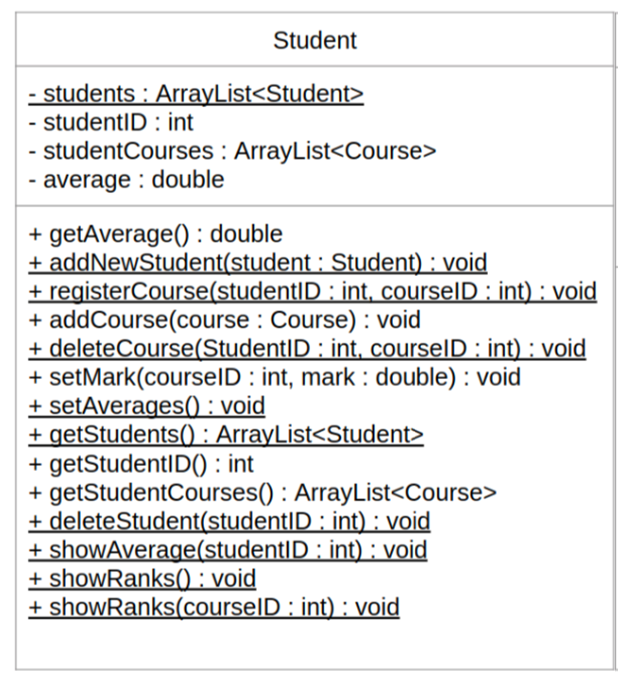
\includegraphics[width=0.49\textwidth ]{uml1.png}	
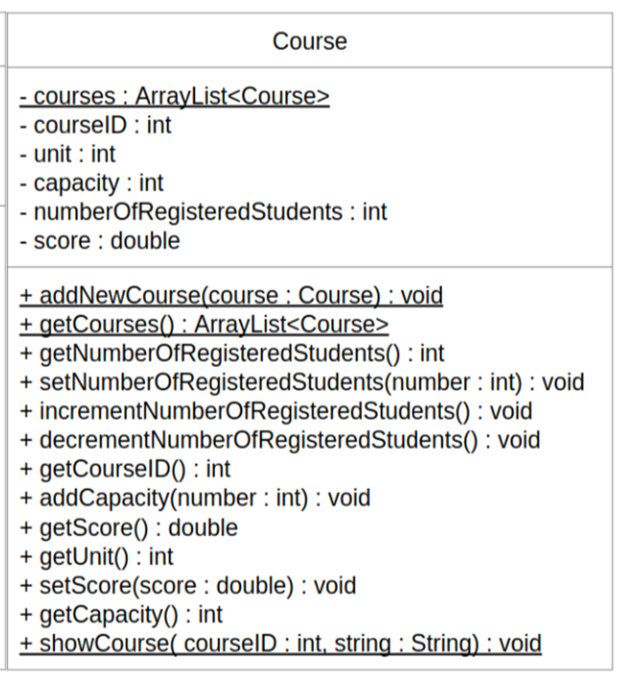
\includegraphics[width=0.49\textwidth ]{uml2.png}
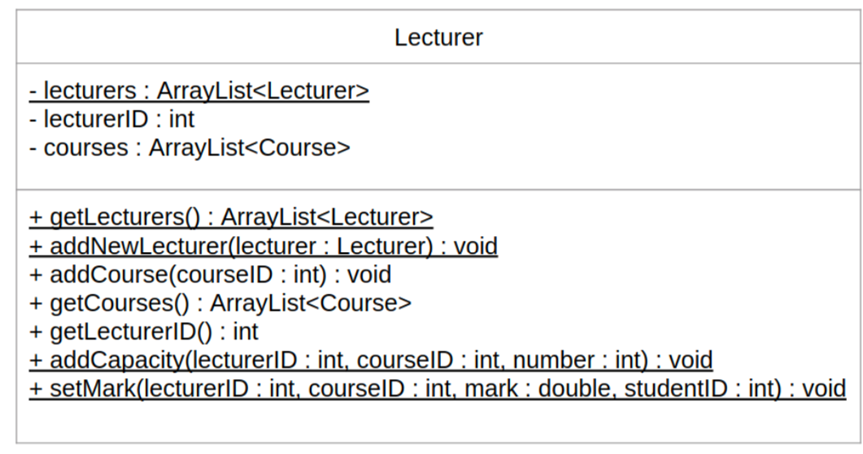
\includegraphics[width=0.8\textwidth ]{uml3.png}
\end{center}
\newpage

\inputsample{
addCourse 40101 3\\
addCourse 40102 4\\
addCourse 40103 4\\
addCourse 40104 3\\
addCourse 25001 4\\
addCourse 25002 3\\
addCourse 25003 4\\
addCourse 65001 3\\
addCourse 65002 3\\
addCourse 65003 4\\
addStudent 95101\\
addStudent 95102\\
addStudent 95103\\
addStudent 95103\\
addStudent 95104\\
addStudent 94101\\
addStudent 94102\\
addStudent 94103\\
addLecturer 10001 40101 40103\\
addLecturer 10002 40102 40104\\
addLecturer 10003 25001 25002\\
addLecturer 10004 65001 65002 65003\\
start semester\\
95101 register 40101 40102 40103 25001 25002\\
95102 register 40101 40102 40103 25001 25002\\
95103 register 40101 40102 40103 25001 25002\\
95104 register 40101 40102 40103 25002 65002\\
94101 register 40102 40103 25001 25002 65001\\
94102 register 40102 40103 25001 25002 65001\\
94103 register 40102 40103 25001 65001\\
end registration\\
10001 mark 40101 95101 12 95102 18 95103 18.5 95104 9.9\\
10002 mark 40102 95101 19.8 95102 20 95103 16.5 95104 19 94101 17 94102 10 94102 15.9\\
10001 mark 40103 95101 17.4 95102 19 95103 15.7 95104 11.2
94101 19 94102 17.8 94103 20\\
10003 mark 25001 95101 9 95102 10 95103 10 94101 10 94102 \\
19 94103 12\\
10003 mark 25002 95101 20 95102 14 95103 18 95104 9.5 
94101 20 94102 18 94103 19.6\\
10004 mark 65001 94101 18 94102 10 94103 15\\
W 40101 95101\\
end semester\\
showAverage 95103\\
showCourse 25001 average\\
showRanks 65001\\
endShow 
}

\outputsample{
15.5\\
11.7\\
94102 94103 94101 	
}
\newpage
\section{‌بازی سزار}
سزار پس از پیروزی بر دشمنان خود (با کمک برنامه ی رمزنگار شما) حوصله اش سر رفته و دنبال یک بازی است. او عاشق بازی \lr{tic tac toe} یا همان ایکس-او است برای همین از شما خواهش کرده است تا یک بازی ایکس-او برایش بنویسید منتها با قوانین خودش.\\
ایکس-او سزار مانند ایکس-او های معمولی یک جدول ۳*۳ است با این تفاوت که درون هر کدام از خانه های جدول یک جدول دیگر نیز قرار دارد!\\
\begin{center}
	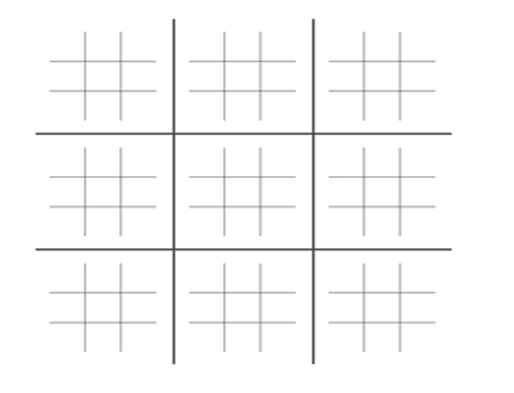
\includegraphics[width=0.8\textwidth ]{cezar1.png}
\end{center}
\newpage
قوانین این بازی به این صورت است که بازیکن اول (در حقیقت حرکت اول) در هرکدام از این خانه ها حرکت خود را انجام می دهد اما بازیکن دوم موظف است تا در همان خانه ای که بازیکن اول بازی خود را شروع کرده اما در جدول «بزرگ» به بازی خود ادامه دهد. به شکل زیر: (یعنی بازیکن دوم حتما باید حرکت خود را در خانه ی های-لایت شده ادامه دهد)\\
\begin{center}
	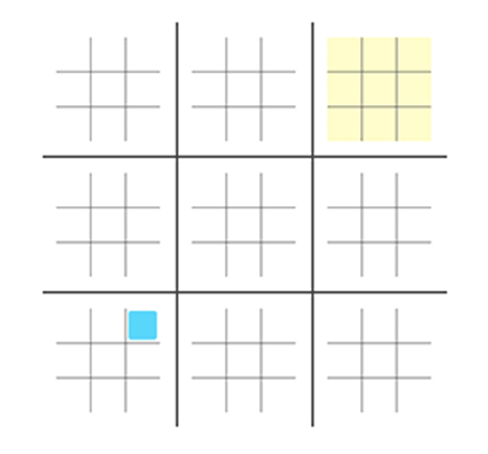
\includegraphics[width=0.8\textwidth ]{cezar2.png}
\end{center}
\newpage
بازی در خانه های کوچک ادامه پیدا میکند تا زمانی که در خانه های کوچک یکی از بازیکن ها برنده میشود و آن خانه متعلق به آن بازیکن می شود.\\

\begin{center}
	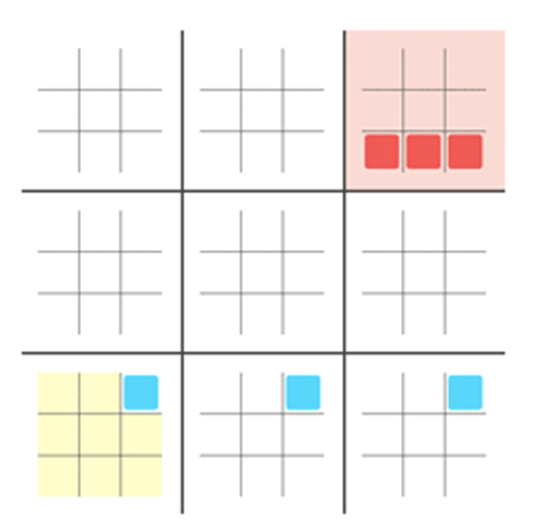
\includegraphics[width=0.8\textwidth ]{cezar3.png}
\end{center}


\textbf{قوانین اضافه::}
\\\\اگر آن خانه ی کوچک که شما باید در آن بازی کنید تکلیفش  مشخص شده باشد آنگاه انتخاب با شماست تا در کدام خانه بازی کنید\\
اگر یکی از خانه های کوچک جدول مساوی شده باشد برای هیچ کدام از بازیکن ها حساب نمیشود و بازی ادامه پیدا میکند.\\
برای آشنایی بیشتر میتوانید این لینک را مشاهده کنید :
 \href{http://bejofo.net/ttt}{(لینک)}
\newpage
البته بازی‌ای که باید بنویسید، صرفا خود بازی ایکس-او نیست. بلکه باید مکانیزم حساب کاربری و ثبت نام و لاگین و… را مطابق مواردی که در ادامه برای شما گفته می شود، پیاده سازی کنید.
در این برنامه، در اصل سه منو (Menu) داریم. یکی منوی ابتدای بازی یا منوی ثبت نام است. یکی منوی اصلی و یکی هم منوی خود بازی. در ادامه به توضیح دستوراتی که در هر کدام از این منوها وارد می شود می پردازیم. توجه کنید که در هنگام شروع برنامه، به طور پیش فرض، کاربر در منوی ثبت نام قرار دارد. در تمامی منوها دستور help وجود دارد که توضیح آن را در هر منو قرار داده ایم. ضمنا توجه کنید تمامی پیغام های انجام موفقیت آمیز دستورات یا خطاها، در یک خط مجزا چاپ می شوند و بعد به خط بعدی می رود.


\hrulefill

\textbf{منوی ثبت نام}
\\\\در ابتدای شروع برنامه کاربر در این منو قرار دارد.
\begin{tcolorbox}[boxrule=0pt]
	\begin{latin}
  	  \large{
  	  	register [username] [password]
		}
	\end{latin}
\end{tcolorbox}
همان طور که مشخص است، یک کاربر با نام کاربری و پسورد مشخص شده را ایجاد می کند. نام کاربری و پسورد باید فقط شامل حروف الفبای انگلیسی، اعداد و کاراکتر آندرلاین  باشند. خطاهای مربوط به این دستور به این ترتیب چک می شوند و هر خطا که رخ داده بود، پیغام همان خطا چاپ شده و سایر خطاها بررسی نمی شوند. اگر هیچ خطایی رخ نداد و عملیات موفقیت آمیز بود، پیغام
\begin{tcolorbox}[boxrule=0pt]
	\begin{latin}
  	  \large{
  	  	register successful
		}
	\end{latin}
\end{tcolorbox}

چاپ خواهد شد.\\


خطاها:
\\اگر نام کاربری شامل کاراکترهایی به جز کاراکترهای ذکر شده بود، پیغام
\begin{tcolorbox}[boxrule=0pt]
	\begin{latin}
  	  \large{
  	  	username format is invalid
		}
	\end{latin}
\end{tcolorbox}
\newpage
اگر پسورد شامل کاراکترهایی به جز کاراکترهای ذکر شده بود، پیغام
\begin{tcolorbox}[boxrule=0pt]
	\begin{latin}
  	  \large{
  	  	password format is invalid
		}
	\end{latin}
\end{tcolorbox}
اگر کاربری با username گفته شده از قبل وجود داشت پیغام

\begin{tcolorbox}[boxrule=0pt]
	\begin{latin}
		\large{
			a user exists with this username
		}
	\end{latin}
\end{tcolorbox}
چاپ خواهد شد.\\

\hrulefill


\begin{tcolorbox}[boxrule=0pt]
	\begin{latin}
  	  \large{
  	  	login [username] [password]
		}
	\end{latin}
\end{tcolorbox}

برای لاگین کردن به حساب کاربری مشخص با نام کاربری و پسورد داده شده استفاده می‌شود. نام کاربری و پسورد باید فقط شامل حروف الفبای انگلیسی، اعداد و کاراکتر آندرلاین \_ باشند. خطاهای مربوط به این دستور به این ترتیب چک می‌شوند و هر خطا که رخ داده بود، پیغام همان خطا چاپ شده و سایر خطاها بررسی نمی‌شوند. اگر هیچ خطایی رخ نداد و عملیات موفقیت‌آمیز بود، پیغام


\begin{tcolorbox}[boxrule=0pt]
	\begin{latin}
  	  \large{
  	  	login successful
		}
	\end{latin}
\end{tcolorbox}

چاپ خواهد شد و پس از آن کاربر به طور خودکار وارد منوی اصلی خواهد شد.

خطاها: 

اگر نام کاربری شامل کاراکترهایی به جز کاراکترهای ذکر شده بود، پیغام:



\begin{tcolorbox}[boxrule=0pt]
	\begin{latin}
  	  \large{
  	  	username format is invalid
		}
	\end{latin}
\end{tcolorbox}

اگر پسورد شامل کاراکترهایی به جز کاراکترهای ذکر شده بود، پیغام:



\begin{tcolorbox}[boxrule=0pt]
	\begin{latin}
  	  \large{
  	  	password format is invalid
		}
	\end{latin}
\end{tcolorbox}

اگر کاربری با username گفته شده وجود نداشت:



\begin{tcolorbox}[boxrule=0pt]
	\begin{latin}
  	  \large{
  	  	no user exists with this username
		}
	\end{latin}
\end{tcolorbox}

اگر پسورد غلط بود:


\begin{tcolorbox}[boxrule=0pt]
	\begin{latin}
  	  \large{
  	  	incorrect password
		}
	\end{latin}
\end{tcolorbox}

چاپ خواهد شد.

\hrulefill




\begin{tcolorbox}[boxrule=0pt]
	\begin{latin}
  	  \large{
  	  	remove [username] [password]
		}
	\end{latin}
\end{tcolorbox}

برای حذف کردن یک حساب کاربری مشخص با نام کاربری و پسورد داده شده استفاده می‌شود. نام کاربری و پسورد باید فقط شامل حروف الفبای انگلیسی، اعداد و کاراکتر آندرلاین \_ باشند. خطاهای مربوط به این دستور به این ترتیب چک می‌شوند و هر خطا که رخ داده بود، پیغام همان خطا چاپ شده و سایر خطاها بررسی نمی‌شوند. اگر همه موفق آمیز بودند پیغام


\begin{tcolorbox}[boxrule=0pt]
	\begin{latin}
  	  \large{
  	  	removed [username] successfully
		}
	\end{latin}
\end{tcolorbox}

چاپ خواهد شد که به جای username باید نام کاربری فرد حذف شده نشان داده شود.

خطاها: 

اگر نام کاربری شامل کاراکترهایی به جز کاراکترهای ذکر شده بود، پیغام:



\begin{tcolorbox}[boxrule=0pt]
	\begin{latin}
  	  \large{
  	  	username format is invalid
		}
	\end{latin}
\end{tcolorbox}

اگر پسورد شامل کاراکترهایی به جز کاراکترهای ذکر شده بود، پیغام:


\begin{tcolorbox}[boxrule=0pt]
	\begin{latin}
  	  \large{
  	  	password format is invalid
		}
	\end{latin}
\end{tcolorbox}

اگر کاربری با username گفته شده وجود نداشت:


\begin{tcolorbox}[boxrule=0pt]
	\begin{latin}
  	  \large{
  	  	no user exists with this username
		}
	\end{latin}
\end{tcolorbox}

اگر پسورد غلط بود:



\begin{tcolorbox}[boxrule=0pt]
	\begin{latin}
  	  \large{
  	  	incorrect password
		}
	\end{latin}
\end{tcolorbox}

چاپ خواهد شد.

\hrulefill




\begin{tcolorbox}[boxrule=0pt]
	\begin{latin}
  	  \large{
  	  	list\_users
		}
	\end{latin}
\end{tcolorbox}

این دستور لیست تمامی کاربرانی که وجود دارند را به ترتیب الفبایی (Lexicographical) نمایش می‌دهد.


\hrulefill



\begin{tcolorbox}[boxrule=0pt]
	\begin{latin}
  	  \large{
  	  	help
		}
	\end{latin}
\end{tcolorbox}

این فرمان انواع دستوراتی که در این بخش قابل نمایش هستند را نمایش می‌دهد. از این دستور صرفاً برای اطمینان حاصل کردن از این که در منوی درست قرار دارید. خروجی این دستور در این منو به صورت زیر است:



\begin{tcolorbox}[boxrule=0pt]
	\begin{latin}
  	  \large{
  	  	register [username] [password]
  	  	
login [username] [password]

remove [username] [password]

list\_users

help

exit
		}
	\end{latin}
\end{tcolorbox}

\hrulefill




\begin{tcolorbox}[boxrule=0pt]
	\begin{latin}
  	  \large{
  	  	exit
		}
	\end{latin}
\end{tcolorbox}

بیانگر اتمام اجرای برنامه است و بعد از چاپ پیام



\begin{tcolorbox}[boxrule=0pt]
	\begin{latin}
  	  \large{
  	  	program ended
		}
	\end{latin}
\end{tcolorbox}

اجرای برنامه پایان می‌پذیرد.

\hrulefill

\textbf{منوی اصلی:}

همان طور که گفته شد، در صورت موفقیت‌آمیز بودن login وارد این منو خواهید شد.

دستورات:

\begin{tcolorbox}[boxrule=0pt]
	\begin{latin}
  	  \large{
  	  	new\_game [username] [limit]
		}
	\end{latin}
\end{tcolorbox}

با این دستور یک بازی جدید شروع می شود. در این بخش باید username یک کاربر دیگر وارد شود و بدین ترتیب بازی با آن کاربر شروع خواهد شد. کاربری که اکنون لاگین کرده و دستور را زده است در حین بازی به عنوان X و بازیکنی که در این دستور نام او وارد شده به عنوان O خوهد بود. Limit هم یک عدد است و بیانگر محدودیت تعداد حرکات (نوبت بازی) است.  اگر این عدد 0 باشد به معنی نبودن هیچ محدودیتی در بازی است. در بخش مربوط به limit جزئیات بیشتر این دستور را توضیح خواهیم داد. 

خطاهای این دستور:

اگر username از کاراکترهایی که در منوی لاگین توضیح دادیم تشکیل نشده بود، پیام:

\begin{tcolorbox}[boxrule=0pt]
	\begin{latin}
  	  \large{
  	  	username format is invalid
		}
	\end{latin}
\end{tcolorbox}



اگر limit عددی کوچک‌تر از 0 بود:

\begin{tcolorbox}[boxrule=0pt]
	\begin{latin}
  	  \large{
  	  	number should be positive to have a limit or 0 for no limit
		}
	\end{latin}
\end{tcolorbox}



اگر کاربری که دستور را زده است، نام کاربری خودش را وارد کرد:

\begin{tcolorbox}[boxrule=0pt]
	\begin{latin}
  	  \large{
  	  	you must choose another player to start a game
		}
	\end{latin}
\end{tcolorbox}



اگر کاربری با این نام کاربری وجود نداشت:

\begin{tcolorbox}[boxrule=0pt]
	\begin{latin}
  	  \large{
  	  	no user exists with this username
		}
	\end{latin}
\end{tcolorbox}



چاپ خواهد شد.

در صورت اجرای موفقیت‌آمیز دستور، پیام:

\begin{tcolorbox}[boxrule=0pt]
	\begin{latin}
  	  \large{
  	  	new game started successfully between [first] and [second] with limit [limit]
		}
	\end{latin}
\end{tcolorbox}



جاپ می‌شود که در آن first نام کاربری بازیکن X و second نام کاربری بازیکن O و limit هم عدد محدودیت بازی است (در حالتی که 0 وارد شده بود \- به معنی عدم محدودیت\- هم عدد 0 نمایش داده خواهد شد و استثنایی وجود ندارد.)

\hrulefill


\begin{tcolorbox}[boxrule=0pt]
	\begin{latin}
  	  \large{
  	  	scoreboard
		}
	\end{latin}
\end{tcolorbox}



پیش از توضیح خروجی این دستور باید در مورد امتیاز دهی در بازی صحبت بکنیم. هر برد معمولی (از طریق زدن شاه) 3 امتیاز و باخت به این شکل 0 امتیاز دارد. در صورتی که یکی از بازیکنان انصراف بدهد (با دستوری که در بخش مربوط به بازی توضیح می‌دهیم)، برنده بازی 2 امتیاز دریافت کرده و شخصی که انصراف داده 1 امتیاز منفی کسب می‌کند. در صورت تساوی بازی (که در اثر اتمام limit اتفاق می‌افتد) هر بازیکن 1 امتیاز می‌گیرد.

 بعد از اجرای این دستور باید کاربران با این فرمت نوشته بشوند:

\begin{tcolorbox}[boxrule=0pt]
	\begin{latin}
  	  \large{
  	  	[username] [score] [wins] [draws] [losses]
		}
	\end{latin}
\end{tcolorbox}



منظور از wins و draws و losses تعداد بردها، تساوی‌ها و باخت هاست.

ترتیب مرتب سازی کاربران هم به ترتیب از بالاترین اولویت به کمترین به این صورت است: بیش‌ترین امتیاز \- در صورت برابری امتیاز بیش‌ترین تعداد برد \- در صورت برابری تعداد برد بیش‌ترین تعداد تساوی \- در صورت برابری تساوی کمترین باخت و در صورت برابری تمامی موارد، براساس حروف الفبا (lexicographical) به طور صعودی (یعنی a زودتر از z می‌آید و…)


\hrulefill





\begin{tcolorbox}[boxrule=0pt]
	\begin{latin}
  	  \large{
  	  	list\_users
		}
	\end{latin}
\end{tcolorbox}

کاملاً مشابه همین دستور که در منوی قبلی توضیح داده شد، عمل می‌کند.

\hrulefill


\begin{tcolorbox}[boxrule=0pt]
	\begin{latin}
  	  \large{
  	  	help
		}
	\end{latin}
\end{tcolorbox}

مشابه همان چیزی است که در بخش قبل توضیح دادیم. خروجی آن عیناً به این شکل است:



\begin{tcolorbox}[boxrule=0pt]
	\begin{latin}
  	  \large{

  	  	new\_game [username] [limit]

scoreboard

list\_users

help

logout
		}
	\end{latin}
\end{tcolorbox}


\hrulefill




\begin{tcolorbox}[boxrule=0pt]
	\begin{latin}
  	  \large{
  	  	logout
		}
	\end{latin}
\end{tcolorbox}

با این دستور کاربر از حساب کاربری خود خارج می‌شود. پس از اجرای این دستور پیام


\begin{tcolorbox}[boxrule=0pt]
	\begin{latin}
  	  \large{
  	  	logout successful
		}
	\end{latin}
\end{tcolorbox}

چاپ شده و کاربر وارد منوی ثبت نام که پیش‌تر توضیح دادیم، می‌شود.

\newpage
\textbf{منوی بازی:}
\\(فرض کنید نفر اول دایره با علامت O و نفر دوم ضربدر با علامت X است)

\begin{tcolorbox}[boxrule=0pt]
	\begin{latin}
  	  \large{
  	  	select board [x]
		}
	\end{latin}
\end{tcolorbox}

این دستور یکی از ۹ زمین کوچک تر بازی را انتخاب می کند ، زمین ها از سمت چپ از ۱ تا ۹ شماره گذاری شده اند.


 خطاهای این دستور:

 اگر مختصات به طور کلی از محدوده خارج بود (یعنی در بازه 1 تا 9 نبود) پیغام:
\begin{tcolorbox}[boxrule=0pt]
	\begin{latin}
  	  \large{
  	  	wrong coordination
		}
	\end{latin}
\end{tcolorbox}
در صورتی که بازی جدول انتخاب شده تمام شده باشد و یکی از دو بازیکن ان را برده باشد پیغام:
\begin{tcolorbox}[boxrule=0pt]
	\begin{latin}
  	  \large{
  	  	[player\_name] has already won on this board
		}
	\end{latin}
\end{tcolorbox}
در صورتی که جدول انتخاب شده مساوی شده باشد پیغام:
\begin{tcolorbox}[boxrule=0pt]
	\begin{latin}
  	  \large{
  	  	this board is tie
		}
	\end{latin}
\end{tcolorbox}
چاپ می شود\\
دقت کنید که در اکثر  دقت کنید که در اکثر حالات بردی که کاربر باید در ان بازی کند فقط یک برد خاص است اما 
کاربر می تواند برد های خالی دیگر را هم انتخاب کند و دستور select اروری نمی دهد.

\hrulefill

\begin{tcolorbox}[boxrule=0pt]
	\begin{latin}
  	  \large{
  	  	deselect
		}
	\end{latin}
\end{tcolorbox}

این دستور برد انتخاب شده را از حالت انتخاب شده خارج می کند.\\
خطای دستور:\\
در صورتی که بردی انتخاب نشده باشد پیغام:


\begin{tcolorbox}[boxrule=0pt]
	\begin{latin}
  	  \large{
  	  	no board is selected
		}
	\end{latin}
\end{tcolorbox}
چاپ می‌شود.
(دقت کنید که بعد از اتمام نوبت هر فرد به صورت پیش فرض زمین بازی برد انتخاب شده ندارد)
\newpage
\begin{tcolorbox}[boxrule=0pt]
	\begin{latin}
  	  \large{
  	  	put mark [x]
		}
	\end{latin}
\end{tcolorbox}
این دستوردر خانه x برد انتخاب شده علامت بازیکن (ایکس یا او) را می گذارد\\
در صورتی که بردی انتخاب نشده باشد پیغام:
\begin{tcolorbox}[boxrule=0pt]
	\begin{latin}
  	  \large{
  	  	no board selected
		}
	\end{latin}
\end{tcolorbox}

چاپ می شود.\\
در صورتی که با گذاشتن علامت بازیکن جدول را ببرد پیغام:
\begin{tcolorbox}[boxrule=0pt]
	\begin{latin}
		\large{
			board [board\_number] won by [player\_name]
		}
	\end{latin}
\end{tcolorbox}
چاپ می شود.\\
در صورتی که با گذاشتن علامت برد بدون بردن کسی پر شود پیغام:

\begin{tcolorbox}[boxrule=0pt]
	\begin{latin}
		\large{
			board [board\_number] is a tie
		}
	\end{latin}
\end{tcolorbox}
چاپ می شود.\\
خطاهای این دستور:

در صورتی که در خانه ی موردنظر علامتی وجود داشت و یا براساس قوانین توضیح داده شده نمی توانستیم در آن برد علامت بگذاریم  پیغام:

\begin{tcolorbox}[boxrule=0pt]
	\begin{latin}
  	  \large{
  	  	cannot put mark here
		}
	\end{latin}
\end{tcolorbox}
چاپ می شود.

\hrulefill

\begin{tcolorbox}[boxrule=0pt]
	\begin{latin}
  	  \large{
  	  	next turn
		}
	\end{latin}
\end{tcolorbox}

نوبت را به حریف منتقل می‌کند و در صورت اجرای موفقت آمیز پیغام:



\begin{tcolorbox}[boxrule=0pt]
	\begin{latin}
  	  \large{
  	  	turn completed
		}
	\end{latin}
\end{tcolorbox}

چاپ می‌شود. توجه کنید که طبق قوانین شطرنج هر نفر باید در نوبت خود حتماً یک حرکت انجام بدهد. بنابراین اگر هیچ حرکتی انجام نشده بود، پیغام خطای:



\begin{tcolorbox}[boxrule=0pt]
	\begin{latin}
  	  \large{
  	  	you must move then proceed to next turn
		}
	\end{latin}
\end{tcolorbox}

نوشته شود.

\hrulefill


\begin{tcolorbox}[boxrule=0pt]
	\begin{latin}
  	  \large{
  	  	show turn
		}
	\end{latin}
\end{tcolorbox}

این دستور برای مشخص شدن این است که نوبت کدام بازیکن است. خروجی آن به فرم زیر است:



\begin{tcolorbox}[boxrule=0pt]
	\begin{latin}
  	  \large{
  	  	its player [player\_name] turn with mark [player\_mark]
		}
	\end{latin}
\end{tcolorbox}


\hrulefill



\begin{tcolorbox}[boxrule=0pt]
	\begin{latin}
  	  \large{
  	  	undo
		}
	\end{latin}
\end{tcolorbox}

یکی از ویژگی‌های منحصر به فرد شطرنجی که باید پیاده سازی کنید، قابلیت undo است. هر بازیکن در کل طول یک بازی می‌تواند دو بار از این قابلیت و در هر نوبت حداکثر یک بار استفاده کند. این قابلیت بدین صورت است که اگر بازیکنی حرکتی انجام داده باشد، در صورتی که بخواهد و طبق شرایط بالا تعداد دفعات استفاده‌اش تمام نشده باشد، حرکت خود را برگرداند. توجه کنید که چون تغییر نوبت با next\_turn انجام می‌شود، همچنان بعد از حرکت نوبت با بازیکن فعلی است تا زمانی که دستور next\_turn زده شود.

خطاهای این دستور:

اگر پیش‌تر به اندازه تعداد کل undo های مجاز (یعنی 2) بار از این قابلیت استفاده شده باشد.


\begin{tcolorbox}[boxrule=0pt]
	\begin{latin}
  	  \large{
  	  	you cannot undo anymore
		}
	\end{latin}
\end{tcolorbox}

اگر بازیکن در این نوبت حرکتی انجام نداده باشد که بخواهد undo کند:


\begin{tcolorbox}[boxrule=0pt]
	\begin{latin}
  	  \large{
  	  	you must move before undo
		}
	\end{latin}
\end{tcolorbox}

اگر در همین نوبت از undo استفاده کرده باشد:



\begin{tcolorbox}[boxrule=0pt]
	\begin{latin}
  	  \large{
  	  	you have used your undo for this turn
		}
	\end{latin}
\end{tcolorbox}

چاپ خواهند شد.

در صورت اجرای درست دستور نیز باید عبارت:


\begin{tcolorbox}[boxrule=0pt]
	\begin{latin}
  	  \large{
  	  	undo completed
		}
	\end{latin}
\end{tcolorbox}

چاپ بشود.

توجه کنید که بعد از اجرای undo، مهره‌ای که از قبل select شده همچنان در همین حالت باقی می‌ماند.


\hrulefill


\begin{tcolorbox}[boxrule=0pt]
	\begin{latin}
  	  \large{
  	  	undo number
		}
	\end{latin}
\end{tcolorbox}

تعداد دفعات باقی مانده undo یک بازیکن را نشان می‌دهد. در ابتدای بازی این عدد دو است و با انجام حرکت undo کاهش می‌یابد تا در نهایت بعد از دو بار انجام این حرکت، به صفر می‌رسد. فرم پیام خروجی به صورت:


\begin{tcolorbox}[boxrule=0pt]
	\begin{latin}
  	  \large{
  	  	you have [n] undo moves
		}
	\end{latin}
\end{tcolorbox}

خواهد بود که n تعداد undo های باقی مانده است.

\hrulefill


\begin{tcolorbox}[boxrule=0pt]
	\begin{latin}
  	  \large{
  	  	show moves
		}
	\end{latin}
\end{tcolorbox}

این دستور کل حرکاتی که بازیکن فعلی انجام داده است را به فرمت زیر نشان می دهد.

\begin{tcolorbox}[boxrule=0pt]
	\begin{latin}
		\large{
			[player\_mark] [board\_number] [inner\_board\_number]
		}
	\end{latin}
\end{tcolorbox}
منظور از متغیر دوم شماره برد است و متغیر سوم نشان دهنده شماره خانه ی برد است.\\

\hrulefill


\begin{tcolorbox}[boxrule=0pt]
	\begin{latin}
  	  \large{
  	  	show moves -all
		}
	\end{latin}
\end{tcolorbox}

این دستور مشابه دستور قبلی است با این تفاوت که حرکات تمامی بازیکنان را به ترتیب از ابتدای شروع بازی نمایش می دهد.

\hrulefill


\begin{tcolorbox}[boxrule=0pt]
	\begin{latin}
  	  \large{
  	  	show board
		}
	\end{latin}
\end{tcolorbox}

این دستور صفحه ی بازی را به فرمت زیر نشان می دهد ( O نشان دهنده دایره و X نشان دهنده ضرب در وE نشان دهنده خانه خالی است)

\begin{tcolorbox}[boxrule=0pt]
	\begin{latin}
  	  \large{
  	  	E|E|E E|E|E E|E|E  \\
  	  	E|O|E E|O|E E|E|E  \\
  	  	E|E|E E|E|E E|E|E  \\
  	  	E|E|E X|X|X E|E|E  \\
  	  	E|E|E X|X|X E|E|E  \\
  	  	E|E|E X|X|X E|E|E  \\
  	  	E|E|E E|E|E E|E|E  \\
  	  	E|E|E E|E|E E|E|E  \\
  	  	E|E|E E|E|E E|E|E  
		}
	\end{latin}
\end{tcolorbox}
دقت کنید اگر یکی از برد ها توسط یکی از بازیکن ها برنده شده باشد تمام خانه های ان برد علامت ان بازیکن گذاشته شود در صورت مساوی لازم نیست کاری انجام دهید و صرفا برد را نشان دهید

\hrulefill


\begin{tcolorbox}[boxrule=0pt]
	\begin{latin}
  	  \large{
  	  	help
		}
	\end{latin}
\end{tcolorbox}

مشابه دستور help در سایر بخش‌هاست. در این جا باید عیناً این خروجی نمایش داده شود:



\begin{tcolorbox}[boxrule=0pt]
	\begin{latin}
  	  \large{
select board [x]\\
deselect\\
put mark [x]\\
next turn\\
show turn\\
undo\\
undo number\\
show moves [-all]\\
show board\\
forfeit\\
help

		}
	\end{latin}
\end{tcolorbox}

\hrulefill

\newpage

\begin{tcolorbox}[boxrule=0pt]
	\begin{latin}
  	  \large{
  	  	forfeit
		}
	\end{latin}
\end{tcolorbox}

این دستور مربوط به انصراف از بازی می‌شود و بازیکنی که این دستور را وارد کند، بازنده بازی خواهد بود و نفر دیگر برنده بازی خواهد بود. همان طور که بالاتر گفتیم، با این اتفاق، حریف که برنده بازی شده، 2 امتیاز می‌گیرد و کسی که انصراف داده منفی 1 امتیاز دریافت می‌کند (یعنی 1 امتیاز از او کم می‌شود).

بعد از اجرای این دستور باید این دو پیام در دو خط پشت سرهم نمایش داده شوند:



\begin{tcolorbox}[boxrule=0pt]
	\begin{latin}
  	  \large{
  	  	you have forfeited
		}
	\end{latin}
\end{tcolorbox}


\begin{tcolorbox}[boxrule=0pt]
	\begin{latin}
  	  \large{
  	  	player [player\_name] with mark [player\_mark] won
		}
	\end{latin}
\end{tcolorbox}

\hrulefill


در اینجا دستورات منوی بازی تمام می شود به موارد زیر توجه داشته باشید
در صورت برد یکی از بازیکنان که باید بعد از دستور next turn بررسی بشود بازی به پایان می رسد و پیغام زیر نمایش داده می شود.



\begin{tcolorbox}[boxrule=0pt]
	\begin{latin}
  	  \large{
  	  	player [player\_name] with mark [player\_mark] wonn
		}
	\end{latin}
\end{tcolorbox}

اگر تمام خانه های بازی پر شود و کسی برنده نشود بازی به پایان می رسد و دستور زیر چاپ می شود.

\begin{tcolorbox}[boxrule=0pt]
	\begin{latin}
  	  \large{
  	  	draw
		}
	\end{latin}
\end{tcolorbox}

و کاربر به منو اصلی باز گردانده می‌شود.

همان طور که پیش‌تر هم گفتیم، در اثر تساوی به هر کدام از بازیکنان 1 امتیاز داده می‌شود.

\hrulefill

اگر در هر کدام از منو ها دستوری زده شد که با قالب دستور های همان منو نمی خواند پیغام زیر چاپ شود



\begin{tcolorbox}[boxrule=0pt]
	\begin{latin}
  	  \large{
  	  	invalid command
		}
	\end{latin}
\end{tcolorbox}

در یک خط چاپ شود و به خط بعدی برویم.

دقت داشته باشید اگر خطای مربوطه یکی از خطاهای دستورات آن منو باشد دیگر این پیغام چاپ نشود و پیغام مربوطه به خطا چاپ شود

در مورد خطاهای دستورات، توجه کنید که ترتیب چک شدن آن‌ها به ترتیبی است که در این مستند نوشته شده‌اند و در صورت رخ دادن اولین خطا و چاپ پیام خطا، سایر خطاها بررسی نمی‌شوند.

\inputsample{
	register ceaser 1234\\
	register decimus 1234\\
	register brutus 1234\\
	register  ali*\& 1234\\
	register ceaser 1234\\
	login amir 1234\\
	remove decimus 1234\\
	login decimus 1234\\
	register decimus 1234\\
	list\_users\\
	help\\
	login ceaser 1234\\
	new\_game amir 0\\
	new\_game amir -100\\
	new\_game brutus 0\\
	select board 1\\
	put mark 5\\
	next turn\\
	put mark 5\\
	select board 5\\
	put mark 3\\
	show board\\
	next turn\\
	select board 3\\
	put mark 5\\
	next turn\\
	show turn\\
	next turn\\
	select board 5\\
	put mark 7\\
	next turn\\
	select board 7\\
	put mark 5\\
	next turn\\
	select board 5\\
	put mark 5\\
	next turn\\
	show moves\\
	show moves -all\\
	show board\\
	forfeit\\
	scoreboard\\
	logout\\
	exit	
}

\outputsample{
register successful\\
register successful\\
register successful\\
username format is invalid\\
a user exists with this username\\
no user exists with this username\\
removed decimus successfully\\
no user exists with this username\\
register successful\\
brutus\\
ceaser\\
decimus\\
register [username] [password]\\
login [username] [password]\\
remove [username] [password]\\
list\_users\\
help\\
exit\\
login successful\\
no user exists with this username\\
number should be positive to have a limit or 0 for no limit\\
new game started successfully between ceaser and brutus with limit 0\\
turn completed\\
no board selected\\
E|E|E E|E|E E|E|E\\
E|O|E E|E|E E|E|E\\
E|E|E E|E|E E|E|E\\
E|E|E E|E|X E|E|E\\ 
E|E|E E|E|E E|E|E\\
E|E|E E|E|E E|E|E\\
E|E|E E|E|E E|E|E\\ 
E|E|E E|E|E E|E|E\\ 
E|E|E E|E|E E|E|E\\
turn completed\\
turn completed\\
its player ceaser turn with mark X\\
you must play then proceed to next turn\\
turn completed\\
turn completed\\
board 5 won by ceaser\\
turn completed\\
O 1 5\\
O 3 5\\
O 7 5\\
O 1 5\\
X 5 3\\
O 3 5\\
X 5 7\\
O 7 5\\
X 5 5\\
E|E|E E|E|E E|E|E\\ 
E|O|E E|E|E E|O|E\\ 
E|E|E E|E|E E|E|E\\
E|E|E X|X|X E|E|E\\ 
E|E|E X|X|X E|E|E\\ 
E|E|E X|X|X E|E|E\\
E|E|E E|E|E E|E|E\\ 
E|O|E E|E|E E|E|E\\ 
E|E|E E|E|E E|E|E\\
you have forfeited\\
player ceaser with mark X won\\
ceaser 2 1 0 0\\
decimus 0 0 0 0\\
brutus -1 0 0 1\\
logout successful\\
program ended 	
}

\newpage
\section{فیفا 21}
در اﯾﻦ ﺳﻮال‪ ،‬ﺑﺎﯾﺪ ﯾﮏ ﻟﯿﮓ ﻓﻮﺗﺒﺎل (ﻣﺎﻧﻨﺪ ﺑﺎزی ﻓﯿﻔﺎ) را ﭘﯿﺎده ﺳﺎزی ﮐﻨﯿﺪ‪ .‬در اﯾﻦ ﻟﯿﮓ‪ ،‬ﺗﻌﺪادی ﺗﯿﻢ وﺟﻮد دارد ﮐﻪ ﻫﺮ ﺗﯿﻢ از‬ ‫ﭼﻨﺪ ﺑﺎزﯾﮑﻦ ﺗﺸﮑﯿﻞ ﺷﺪه اﺳﺖ‪.‬‬
\\\\
ﻟﯿﮓ‬
\\
‫ﻫﻤﺎنﻃﻮر ﮐﻪ اﺷﺎره ﺷﺪ‪ ،‬در اﯾﻦ ﻟﯿﮓ‪ ،‬ﺗﻌﺪادی ﺗﯿﻢ وﺟﻮد دارد‪ .‬و ﻫﻤﭽﻨﯿﻦ ﺑﺎزﯾﮑﻦﻫﺎﯾﯽ ﮐﻪ ﺗﯿﻢ ﻧﺪارﻧﺪ در ﻟﯿﮓ ﻗﺮار ﻣﯽﮔﯿﺮﻧﺪ‪.‬‬ ‫در واﻗﻊ‪ ،‬ﺗﻤﺎم ﮐﺎرﻫﺎی اﺻﻠﯽ (از ﺟﻤﻠﻪ ﺧﺮﯾﺪ و ﻓﺮوش ﺑﺎزﯾﮑﻦ‪ ،‬اﻧﺠﺎم ﺑﺎزیﻫﺎی دوﺳﺘﺎﻧﻪ‪ ،‬و ﺳﭙﺮی ﮐﺮدن ﯾﮏ ﻓﺼﻞ از ﻟﯿﮓ)در ‫ﺳﺎزﻣﺎن ﻟﯿﮓ اﻧﺠﺎم ﻣﯽﺷﻮد.
\\\\
تیم
\\
‫ﻫﺮ ﺗﯿﻢ‪ ،‬ﯾﮏ ﻧﺎم‪ ،‬ﻣﻘﺪاری ﭘﻮل ﺑﻪ ﻋﻨﻮان ﺑﻮدﺟﻪ‪ ،‬ﯾﮏ ﺗﺮﮐﯿﺐ اﺻﻠﯽ و ﺗﻌﺪادی ﺑﺎزﯾﮑﻦ ذﺧﯿﺮه دارد‪.‬‬
\\\\
‫ﺗﺮﮐﯿﺐ اﺻﻠﯽ(squad)
\\
در ترکیب اصلی ۱۱ بازیکن که قرار است در ﺑﺎزیﻫﺎ ﺣﺎﺿﺮ ﺷﻮﻧﺪ‪ ،‬ﻗﺮار ﻣﯽﮔﯿﺮﻧﺪ‪ .‬ﺑﺮای راحتی کار، تمام ترکیب‌ها از آرایش \lr{4-3-3} برخوردارند؛  ۱‬ دروازهﺑﺎن - ‪ ۴‬ﻣﺪاﻓﻊ ‪ ۳ -‬ﻫﺎﻓﺒﮏ و ۳ مهاجم.
\\\\
ﺑﺎزﯾﮑﻦ
\\
ﻫﺮ ﺑﺎزﯾﮑﻦ‪ ،‬ﻧﺎم‪ ،‬ﻧﺎم ﺧﺎﻧﻮادﮔﯽ‪ ،‬ﺳﻦ‪ ،‬و ﯾﮏ ﻗﺮارداد دارد‪.‬‬
‫‪ ۴‬ﭘﺴﺖ ﻣﺨﺘﻠﻒ ﺑﺮای ﺑﺎزﯾﮑﻦﻫﺎ وﺟﻮد دارد؛ دروازهﺑﺎن‪ ،‬ﻣﺪاﻓﻊ‪ ،‬ﻫﺎﻓﺒﮏ‪ ،‬و ﻣﻬﺎﺟﻢ‪ .‬ﻫﺮ ﺑﺎزﯾﮑﻦ ﺑﻪ ﻧﺴﺒﺖ ﭘﺴﺖ ﺧﻮدش‪ ،‬ﻣﻌﯿﺎرﻫﺎﯾﯽ‬
‫ﺑﺮای ﺳﻨﺠﺶ ﺗﻮاﻧﺎﯾﯽﻫﺎﯾﺶ دارد‪.‬‬
\\\\
‫دروازهﺑﺎن‬
\\
ﻣﻌﯿﺎرﻫﺎی ﻫﺮ دروازهﺑﺎن ﻋﺒﺎرت اﻧﺪ از‪:‬‬
\\
\begin{itemize}
	\item
	ﻗﺪرت ﺷﻮت ﮔﯿﺮی \lr{(Shoot Saving)} 
	\item
	واﮐﻨﺶ ﻧﺸﺎن دادن \lr{‪(Reactions)}‬‬
	\item
	ﭘﻨﺎﻟﺘﯽﮔﯿﺮی \lr{(‪Penalty Saving)}‬‬‫‬
\end{itemize}
مدافع
\\
ﻣﻌﯿﺎرﻫﺎی ﻫﺮ مدافع ﻋﺒﺎرت اﻧﺪ از‪:‬‬
\begin{itemize}
	\item
	‫ ﻗﺪرت ﺑﺪﻧﯽ \lr{(Strength)} 
	\item
	ﺧﺸﻮﻧﺖ \lr{(Aggression)}‬‬‫ 
	\item
	ﺳﺮ زﻧﯽ \lr{(Heading)}‬‬‫
\end{itemize}

ﻫﺎﻓﺒﮏ
\\
‫ﻣﻌﯿﺎرﻫﺎی ﻫﺮ ﻫﺎﻓﺒﮏ ﻋﺒﺎرت اﻧﺪ از‪:‬‬
\begin{itemize}
	\item
	‫ ﭘﺎسﮐﺎری \lr{(Passing)}‬‬‫ 
	\item
	ﺷﻮت زﻧﯽ \lr{(Shooting)}‬‬‫ 
	\item
	ﺳﺎﻧﺘﺮ ﮐﺮدن \lr{(Crossing)}
\end{itemize}
ﻣﻬﺎﺟﻢ
\\
‫ﻣﻌﯿﺎرﻫﺎی ﻫﺮ ﻣﻬﺎﺟﻢ ﻋﺒﺎرت اﻧﺪ از:
\begin{itemize}
	\item
	سر زنی \lr{(Heading)} 
	\item
	تمام کنندگی \lr{(Finishing)} 
	\item
	پنالتی زنی \lr{(Penalties)}
\end{itemize}


ﻫﺮ ﺑﺎزﯾﮑﻦ در زﻣﺎن اﯾﺠﺎد ﺷﺪن (ﭘﯿﻮﺳﺘﻦ ﺑﻪ دﻧﯿﺎی ﻓﻮﺗﺒﺎل)‪ ،‬ﯾﮏ ﺑﺎزﯾﮑﻦ آزاد ﻣﺤﺴﻮب ﻣﯽﺷﻮد‪ .‬زﻣﺎﻧﯽ ﮐﻪ ﺑﺎزﯾﮑﻦ ﺑﻪ ﺗﯿﻤﯽ ﺑﭙﯿﻮﻧﺪد ‫ﻗﺮاردادی اﻣﻀﺎ ﻣﯽﮐﻨﺪ ﮐﻪ در آن ﻗﺮارداد‪ ،‬ﺗﻌﺪاد ﺳﺎلﻫﺎﯾﯽ ﮐﻪ ﺑﺎزﯾﮑﻦ ﺑﺎ آن ﺗﯿﻢ ﻗﺮارداد دارد ذﮐﺮ ﺷﺪه اﺳﺖ‪ .‬ﻫﻤﭽﻨﯿﻦ ﯾﮏ ﻧﻮع ‫ﻗﺮارداد ﻗﺮﺿﯽ ﻧﯿﺰ دارﯾﻢ ﮐﻪ ﯾﮏ ﺑﺎزﯾﮑﻦ در ﺻﻮرﺗﯽ ﮐﻪ در ﯾﮏ ﺗﯿﻢ ﻣﺸﻐﻮل ﺑﻪ ﻓﻌﺎﻟﯿﺖ ﺑﺎﺷﺪ‪ ،‬ﻣﯽ ﺗﻮاﻧﺪ ﺑﺮای ﻣﺪﺗﯽ در ﺗﯿﻤﯽ دﯾﮕﺮ ‫ﺑﺎزی ﮐﻨﺪ و ﭘﺲ از اﺗﻤﺎم ﻗﺮارداد ﻗﺮﺿﯽ‪ ،‬ﺑﻪ ﺗﯿﻢ اوﻟﯿﻪ ﺧﻮد ﺑﺎزﮔﺮدد‪ .‬ﻣﺪت ﻗﺮارداد ﻗﺮﺿﯽ ﻧﺒﺎﯾﺪ از ﻣﺪت ﻗﺮارداد اﺻﻠﯽ ﺑﯿﺸﺘﺮ ﺑﺎﺷﺪ‪.
\\
در ﻫﺮ ﻓﺼﻞ از ﻟﯿﮓ‪ ،‬ﻫﺮ ﺗﯿﻢ ﺑﺎ ﺗﻤﺎم ﺗﯿﻢﻫﺎی دﯾﮕﺮ دو ﺑﺎر ﺑﺎزی ﻣﯽﮐﻨﺪ‪ .‬ﯾﮏ ﺑﺎر در ﺧﺎﻧﻪی ﺧﻮدش و ﺑﺎر دﯾﮕﺮ در ﺧﺎﻧﻪی ﺣﺮﯾﻒ‪ .‬در ‫ﺻﻮرﺗﯽ ﮐﻪ ﺗﯿﻤﯽ در ﯾﮏ ﺑﺎزی ﻣﻬﻤﺎن ﺑﺎﺷﺪ‪ ،‬از ﻣﻌﯿﺎر ﻫﺎی ﻫﺮ ‫ﺑﺎزﯾﮑﻦ آن ‪ ۵‬ﺗﺎ ﮐﻢ ﻣﯽ ﺷﻮد.
\\
ﻫﺮ ﺗﯿﻢ‪ ،‬ﻣﻘﺪاری ﺑﻮدﺟﻪ دارد ﮐﻪ از آن ﺑﺮای ﺧﺮﯾﺪ ﺑﺎزﯾﮑﻦ اﺳﺘﻔﺎده ﻣﯽﮐﻨﺪ‪ .‬ﻫﺰﯾﻨﻪی ﺧﺮﯾﺪ ﺑﺎزﯾﮑﻦﻫﺎ از ﺑﻮدﺟﻪی ﺗﯿﻢ ﻣﻘﺼﺪ ‫ﭘﺮداﺧﺖ ﺷﺪه و ﺑﻪ ﺑﻮدﺟﻪی ﺗﯿﻢ ﻣﺒﺪا وارﯾﺰ ﻣﯽﺷﻮد و ﺑﺎزﯾﮑﻦ ﺧﺮﯾﺪاری ﺷﺪه ﺑﻪ ﻟﯿﺴﺖ ﺑﺎزﯾﮑﻨﺎن ذﺧﯿﺮهی ﺗﯿﻢ ﺟﺪﯾﺪ ﻣﻨﺘﻘﻞ ﻣﯽﺷﻮد‪.‬‬
\\
‫ﺑﻮدﺟﻪی ﺗﯿﻢﻫﺎ و ﻫﺰﯾﻨﻪﻫﺎی ﻣﺸﺨﺺ ﺷﺪه ﻫﻤﮕﯽ ﺑﺮ ﺣﺴﺐ ﻣﯿﻠﯿﻮن دﻻر ﻫﺴﺘﻨﺪ.
\\\\
‫ﻧﺘﯿﺠﻪ ﻫﺮ ﺑﺎزی ﺑﻪ اﯾﻦ ﺻﻮرت ﻣﺤﺎﺳﺒﻪ ﻣﯽﺷﻮد‪:‬‬
\\
\begin{itemize}
	\item
	‫ در ﺻﻮرﺗﯽ ﮐﻪ ﻣﯿﺎﻧﮕﯿﻦ ﻗﺪرت ﭘﺎسﮐﺎری ﻫﺎﻓﺒﮏﻫﺎ از ‪ ۸۵‬ﺑﯿﺸﺘﺮ ﺑﺎﺷﺪ‪ ،‬ﻣﻮﻗﻌﯿﺖ ﻫﺎی ﺑﻬﺘﺮی ﻧﺼﯿﺐ ﻣﻬﺎﺟﻢ ﻫﺎ ﻣﯽﺷﻮد و ﺑﻪ‬‫ﻗﺪرت ﺗﻤﺎمﮐﻨﻨﺪﮔﯽ ﻫﺮ ﻣﻬﺎﺟﻢ ‪ ۵‬ﺗﺎ اﺿﺎﻓﻪ ﻣﯽﺷﻮد‪ .‬ﻫﻤﭽﻨﯿﻦ اﮔﺮ ﻫﺎﻓﺒﮑﯽ در ﺗﯿﻢ ﺑﺎﺷﺪ ﮐﻪ ﻗﺪرت ﭘﺎسﮐﺎریاش از ‪ ۹۰‬ﺑﯿﺸﺘﺮ‬
	‫ﺑﺎﺷﺪ‪ ،‬ﺑﻪ ﻗﺪرت ﺗﻤﺎم ﮐﻨﻨﺪﮔﯽ ﻫﺮ ﻣﻬﺎﺟﻢ ‪ ۵‬ﺗﺎ اﺿﺎﻓﻪ ﻣﯽﺷﻮد‪.‬‬
	\item
	 ‫ در ﺻﻮرﺗﯽ ﮐﻪ ﻣﯿﺎﻧﮕﯿﻦ ﻗﺪرت ﺑﺪﻧﯽ ﻣﺪاﻓﻊﻫﺎی ﺣﺮﯾﻒ از ‪ ۸۵‬ﺑﯿﺸﺘﺮ ﺑﺎﺷﺪ‪ ،‬آنﻫﺎ در ﻣﺼﺎفﻫﺎﯾﯽ ﮐﻪ در ﻣﻘﺎﺑﻞ ﻣﻬﺎﺟﻤﺎن دارﻧﺪ ‬‫ﭘﯿﺮوز ﻣﯽﺷﻮﻧﺪ و از ﻗﺪرت ﺗﻤﺎمﮐﻨﻨﺪﮔﯽ ﻫﺮ ﻣﻬﺎﺟﻢ ‪ ۳‬ﺗﺎ ﮐﻢ ﻣﯽﺷﻮد‪ .‬ﻫﻤﭽﻨﯿﻦ اﮔﺮ ﻣﺪاﻓﻌﯽ در ﺗﯿﻢ ﺑﺎﺷﺪ ﮐﻪ ﻗﺪرت ﺑﺪﻧﯽاش از بیشتر از ۹۰ باشد از قدرت تمام کنندگی هر مهاجم ۳تا کم میشود.‬‬
	\item
	‫ ﺑﻪ ازای ﻫﺮ ﻣﻬﺎﺟﻢ‪ ،‬اﮔﺮ ﻗﺪرت ﺗﻤﺎمﮐﻨﻨﺪﮔﯽ او از ﻗﺪرت واﮐﻨﺶ ﻧﺸﺎن دادن دروازهﺑﺎن ﺣﺮﯾﻒ ﺑﯿﺸﺘﺮ ﺑﺎﺷﺪ‪ ،‬آن ﻣﻬﺎﺟﻢ ﯾﮏ ﮔﻞ‬‫ﺑﻪ ﺛﻤﺮ ﻣﯽرﺳﺎﻧﺪ‪ .‬و اﮔﺮ ﻣﯿﺎﻧﮕﯿﻦ ﻗﺪرت ﺗﻤﺎمﮐﻨﻨﺪﮔﯽ ﻣﻬﺎﺟﻢﻫﺎ از ﻗﺪرت واﮐﻨﺶ ﻧﺸﺎن دادن دروازه ﺑﺎن ﺣﺮﯾﻒ ﺣﺪاﻗﻞ ‪ ۵‬ﺗﺎ ﺑﯿﺸﺘﺮ ﺑﺎﺷﺪ‪ ،‬ﺗﯿﻢ ﺣﻤﻠﻪ ﮐﻨﻨﺪه ‪ ۲‬ﮔﻞ ﺑﻪ ﺛﻤﺮ ﻣﯽرﺳﺎﻧﺪ‪.
	\item
	‫ ﺑﻪ ازای ﻫﺮ ﻫﺎﻓﺒﮏ‪ ،‬اﮔﺮ ﻗﺪرت ﺷﻮت زﻧﯽ او از ﻗﺪرت ﺷﻮتﮔﯿﺮی دروازهﺑﺎن ﺣﺮﯾﻒ ﺑﯿﺸﺘﺮ ﺑﺎﺷﺪ‪ ،‬او ﯾﮏ ﮔﻞ ﺑﻪ ﺛﻤﺮ ﻣﯽرﺳﺎﻧﺪ ‪.‬‬‫ 
	\item
	ﺑﻪ ازای ﻫﺮ ﻣﺪاﻓﻊ ﯾﺎ ﻣﻬﺎﺟﻢ‪ ،‬اﮔﺮ ﻗﺪرت ﺳﺮزﻧﯽ او ﺿﺮب در ﻣﯿﺎﻧﮕﯿﻦ ﻗﺪرت ﺳﺎﻧﺘﺮ ﻫﺎﻓﺒﮏ ﻫﺎ‪ ،‬از ﻣﺠﺬور ﻗﺪرت واﮐﻨﺶ ﻧﺸﺎن‬‫ دادن دروازهﺑﺎن ﺣﺮﯾﻒ ﺑﯿﺸﺘﺮ ﺑﺎﺷﺪ‪ ،‬آن ﺑﺎزﯾﮑﻦ ﯾﮏ ﮔﻞ ﺑﻪ ﺛﻤﺮ ﻣﯽرﺳﺎﻧﺪ‪.‬‬
	\item
	اﮔﺮ ﻣﯿﺎﻧﮕﯿﻦ ﺧﺸﻮﻧﺖ ﻣﺪاﻓﻌﺎن ﺣﺮﯾﻒ از ‪ ۸۵‬ﺑﯿﺸﺘﺮ ﺑﺎﺷﺪ‪ ،‬ﺗﯿﻢ ﺣﻤﻠﻪﮐﻨﻨﺪه ﺻﺎﺣﺐ ﯾﮏ ﺿﺮﺑﻪ ﭘﻨﺎﻟﺘﯽ ﻣﯽﺷﻮد و ﻣﻬﺎﺟﻤﯽ ﮐﻪ‬‫ﺑﯿﺸﺘﺮﯾﻦ ﻗﺪرت ﭘﻨﺎﻟﺘﯽزﻧﯽ را دارد ﭘﺸﺖ ﺗﻮپ ﻣﯽاﯾﺴﺘﺪ‪ .‬در ﺻﻮرﺗﯽ ﮐﻪ ﻗﺪرت ﭘﻨﺎﻟﺘﯽزﻧﯽ او از ﻗﺪرت ﭘﻨﺎﻟﺘﯽﮔﯿﺮی دروازهﺑﺎن ‫ﺣﺮﯾﻒ ﺑﯿﺸﺘﺮ ﺑﺎﺷﺪ‪ ،‬ﭘﻨﺎﻟﺘﯽ ﺗﺒﺪﯾﻞ ﺑﻪ ﮔﻞ ﻣﯽﺷﻮد‪ ،‬و در ﻏﯿﺮ اﯾﻦﺻﻮرت دروازهﺑﺎن ﭘﻨﺎﻟﺘﯽ را ﻣﯽﮔﯿﺮد.
	\item
ﭘﺲ از ﻣﺤﺎﺳﺒﻪی ﺗﻌﺪاد ﮔﻞﻫﺎی ﻫﺮ ﺗﯿﻢ‪ ،‬ﺑﺮﻧﺪه و ﺑﺎزﻧﺪه ی آن ﺑﺎزی (ﯾﺎ ﺗﺴﺎوی ﺗﯿﻢﻫﺎ)ﻣﺸﺨﺺ ﻣﯽﺷﻮد‪ .‬ﻫﺮ ﺑﺮد ‪ ۳‬اﻣﺘﯿﺎز و ﺗﺴﺎوی‬‫‪ ۱‬اﻣﺘﯿﺎز دارد‪ .‬ﺑﺎﺧﺖ ﻫﻢ اﻣﺘﯿﺎزی ﻧﺪارد‪.‬‬
	\item
در اﻧﺘﻬﺎی ﻓﺼﻞ‪ ،‬ﺑﻪ ﺗﯿﻢﻫﺎی اول‪ ،‬دوم و ﺳﻮم ﺑﻪ ﺗﺮﺗﯿﺐ ‪ ۵۰ ،۱۰۰‬و ‪ ۲۰‬ﻣﯿﻠﯿﻮن دﻻر ﭘﺎداش داده ﻣﯽﺷﻮد‪ .‬ﺑﺎزﯾﮑﻨﺎﻧﯽ ﮐﻪ‬‫ﻗﺮاردادﺷﺎن ﺗﻤﺎم ﺷﺪه ﺑﻪ ﻟﯿﺴﺖ ﺑﺎزﯾﮑﻨﺎن آزاد ﻣﻨﺘﻘﻞ ﻣﯽﺷﻮﻧﺪ و ﺑﺎزﯾﮑﻨﺎﻧﯽ ﮐﻪ ﺑﺎ ﻗﺮارداد ﻗﺮﺿﯽ در ﺗﯿﻢ دﯾﮕﺮی ﺑﺎزی ﻣﯽﮐﺮدﻧﺪ ‫ﺑﻪ ﺗﯿﻢ اﺻﻠﯽ ﺑﺎزﻣﯽﮔﺮدﻧﺪ‪ .‬ﻫﻤﭽﻨﯿﻦ ﺳﻦ ﺗﻤﺎم ﺑﺎزﯾﮑﻨﺎن ﯾﮏ ﺳﺎل اﻓﺰاﯾﺶ ﻣﯽﯾﺎﺑﺪ‪ .‬ﺑﺎزﯾﮑﻨﺎﻧﯽ ﮐﻪ ‪ ۴۰‬ﺳﺎل ﯾﺎ ﺑﯿﺸﺘﺮ ﺳﻦ دارﻧﺪ ‫ﺑﺎزﻧﺸﺴﺘﻪ ﺷﺪه و از ﻓﻮﺗﺒﺎل ﺧﺪاﺣﺎﻓﻈﯽ ﻣﯽﮐﻨﻨﺪ‪.‬‬\\\\
	
\end{itemize}

\textbf{‫دﺳﺘﻮرات ورودی‬}
\begin{tcolorbox}[boxrule=0pt]
	\begin{latin}
		\large{
			‫‪create team teamName‬‬
		}
	\end{latin}
\end{tcolorbox}
‫ﯾﮏ ﺗﯿﻢ ﺑﺎ ﻧﺎم ﻣﺸﺨﺺ ﺷﺪه ﻣﯽﺳﺎزد‪ .‬ﺑﻮدﺟﻪی اوﻟﯿﻪی ﺗﯿﻢ ‪ ۱۰۰‬ﻣﯿﻠﯿﻮن دﻻر اﺳﺖ‪.‬‬
\\
‫در ﺻﻮرﺗﯽ ﮐﻪ ﺗﯿﻤﯽ ﺑﺎ اﯾﻦ ﻧﺎم وﺟﻮد داﺷﺘﻪ ﺑﺎﺷﺪ ‪ \lr{a team exists with this name} ‬ﭼﺎپ ﻣﯽﺷﻮد‪.‬‬
\\
‫در ﺻﻮرﺗﯽ ﮐﻪ ﺗﯿﻢ ﺑﺎ ﻣﻮﻓﻘﯿﺖ ﺳﺎﺧﺘﻪ ﺷﻮد ‪ \lr{team created}‬ﭼﺎپ ﻣﯽﺷﻮد‪.‬‬

\hrulefill

\begin{tcolorbox}[boxrule=0pt]
	\begin{latin}
		\large{
			‫‪delete team teamName‬‬
		}
	\end{latin}
\end{tcolorbox}
ﺗﯿﻢ ﻣﻮرد ﻧﻈﺮ را ﻣﻨﺤﻞ ﻣﯽﮐﻨﺪ.‪ \\ ‬در ﺻﻮرﺗﯽ ﮐﻪ ﺗﯿﻤﯽ ﺑﺎ اﯾﻦ ﻧﺎم وﺟﻮد ﻧﺪاﺷﺘﻪﺑﺎﺷﺪ 
‪ \lr{invalid team} ،‬ﭼﺎپ ﻣﯽﺷﻮد‪.‬‬
\\
‫ﭘﺲ از ﺣﺬف ﺗﯿﻢ ﻣﻮرد ﻧﻈﺮ‪ ،‬ﺑﺎزﯾﮑﻨﺎن آن ﺑﻪ ﺑﺎزﯾﮑﻨﺎن آزاد ﻣﻨﺘﻘﻞ ﻣﯽﺷﻮﻧﺪ و ﻗﺮاردادﻫﺎی آنﻫﺎ ﻧﯿﺰ ﻓﺴﺦ ﻣﯽﺷﻮد‪.‬‬

\hrulefill
\begin{tcolorbox}[boxrule=0pt]
	\begin{latin}
		\large{
			‫‪create player firstName lastName age position‬‬
		}
	\end{latin}
\end{tcolorbox}
دﻗﺖ ﮐﻨﯿﺪ ﮐﻪ ‪ \lr{position‬} ﺑﺎﯾﺪ ﺑﺎ ﯾﮑﯽ از ﻋﺒﺎرات GK DF MF ST  باشد.
\\GK = دروازه بان
\\MF = هافبک
\\DF = دفاع
\\ST = مهاجم 
‫\\اﮔﺮ ﺑﺎزﯾﮑﻨﯽ ﺑﺎ اﯾﻦ ﻧﺎم وﺟﻮد داﺷﺘﻪ ﺑﺎﺷﺪ ‪ \lr{a player exists with this name}‬ﭼﺎپ ﻣﯽﺷﻮد‪.‬‬
‫اﮔﺮ ورودی ﻣﺸﮑﻠﯽ ﻧﺪاﺷﺖ‪ ،‬ﺑﻪ ﻧﺴﺒﺖ ﭘﺴﺖ ﺑﺎزﯾﮑﻦ‪ ،‬ﻣﻌﯿﺎرﻫﺎ را درﯾﺎﻓﺖ ﻣﯽﮐﻨﺪ‪ .‬ﺑﻪ اﯾﻦ ﺻﻮرت ﮐﻪ ﺑﻪ ﺗﺮﺗﯿﺐ آورده ﺷﺪه در ﺑﺎﻻ ﻣﻌﯿﺎرﻫﺎ ﭼﺎپ ﻣﯽﺷﻮد و ﻣﻘﺎدﯾﺮ ﻣﻮرد ﻧﻈﺮ از ورودی درﯾﺎﻓﺖ ﻣﯽ ﺷﻮد‪ .‬ﻣﺜﻼ ﺑﺮای ﯾﮏ ﻣﺪاﻓﻊ‪ ،‬ﻋﺒﺎرات زﯾﺮ در ﺧﺮوﺟﯽ ﭼﺎپ ﺷﺪه و‬
‫ﭘﺲ از ﭼﺎپ ﺷﺪن ﻫﺮ ﺧﻂ‪ ،‬ﻣﻘﺪار ﻣﺮﺑﻮﻃﻪ ﺑﺮای ﻫﺮ ﻣﻌﯿﺎر درﯾﺎﻓﺖ ﻣﯽﺷﻮد‪:‬‬
\begin{tcolorbox}[boxrule=0pt]
	\begin{latin}
		\large{
			Strength:‬‬\\
			‫‪Aggression:‬‬\\
			‫‪Heading:‬‬
		}
	\end{latin}
\end{tcolorbox}
‫زﻣﺎﻧﯽ ﮐﻪ ﺑﺎزﯾﮑﻦ ﮐﻪ ﺳﺎﺧﺘﻪ ﺷﺪ ‪ \lr{player created}‬ﭼﺎپ ﺷﺪه و ﺑﺎزﯾﮑﻦ ﺑﻪ ﻟﯿﺴﺖ ﺑﺎزﯾﮑﻦﻫﺎی آزاد ﻣﻨﺘﻘﻞ ﻣﯽﺷﻮد‪.‬‬

\hrulefill

\begin{tcolorbox}[boxrule=0pt]
	\begin{latin}
		\large{
			print free players
		}
	\end{latin}
\end{tcolorbox}

لیست بازیکن های آزاد را ابتدا به بر اساس پست (به ترتیب دروازه بان، مدافع، هافبک، مهاجم) و سپس نام خانوادگی و نام
مرتب کرده و چاپ می کند.
\\
‫ﻣﺜﺎل:
\begin{tcolorbox}[boxrule=0pt]
	\begin{latin}
		\large{
			1. Mohammad Mohammadi GK
			\\
			2. Ali Alavi DF
			\\
			3. Reza Rezaei DF
			\\
			...
		}
	\end{latin}
\end{tcolorbox}

\hrulefill

\begin{tcolorbox}[boxrule=0pt]
	\begin{latin}
		\large{
			move free player firstName lastName to teamName with \#years years 
			contract
		}
	\end{latin}
\end{tcolorbox}

در ﺻﻮرﺗﯽ ﮐﻪ ﺗﯿﻢ ﯾﺎﻓﺖ ﻧﺸﻮد‬‬‬ \lr{invalid team} چاپ ﻣﯽﺷﻮد.
\\
در ﺻﻮرﺗﯽ ﮐﻪ ﺑﺎزﯾﮑﻦ آزاد ﻣﻮرد ﻧﻈﺮ ﯾﺎﻓﺖ ﻧﺸﻮد \lr{invalid free player} ﭼﺎپ 
ﻣﯽﺷﻮد.
\\
در ﺻﻮرت ﻗﺎﺑﻞ ﻗﺒﻮل ﺑﻮدن ورودیﻫﺎ‬‬‬‬، ﺑﺎزﯾﮑﻦ آزاد ﻣﻮرد ﻧﻈﺮ ﺑﺎ ﻗﺮارداد‬ 
\lr{years} ساله به تیم مشخص شده منتقل ﻣﯽﺷﻮد و ﭘﯿﺎم \lr{free player moved} ﭼﺎپ 
ﻣﯽﺷﻮد.

\hrulefill

\begin{tcolorbox}[boxrule=0pt]
	\begin{latin}
		\large{
			print stats of team teamName
		}
	\end{latin}
\end{tcolorbox}

مشخصات یک تیم از جمله نام تیم، بودجه ی آن، و بازیکنان اصلی و ذخیره آن 
تیم را چاپ می کند. در صورتی که تیم یافت نشود \lr{invalid team} ﭼﺎپ ﻣﯽﺷﻮد. 
\\
ترتیب بازیکن ها باید بر اساس پست(دروازه بان، مدافع، هافبک، مهاجم)، و 
سپس نام خانوادگی و نام مرتب شود.
\begin{tcolorbox}[boxrule=0pt]
	\begin{latin}
		\large{
			
			Team: Chelsea\\
			Budget: 100\\
			Squad players:\\
			1. Kepa Arrizabalaga GK Age: 24 Contract: 6 years\\
			2. Marcos Alonso DF Age: 28 Contract: 4 years\\
			3. Cesar Azpilicueta DF Age: 29 Contract: 3 years\\
			Reserve players:\\
			1. Willy Caballero GK Age: 37 Contract: 1 years\\
			2. Gary Cahill DF Age: 33 Contract: 1 years
			
		}
	\end{latin}
\end{tcolorbox}

\hrulefill

\begin{tcolorbox}[boxrule=0pt]
	\begin{latin}
		\large{
			print stats of player firstName lastName
		}
	\end{latin}
\end{tcolorbox}

ﻣﺸﺨﺼﺎت ﯾﮏ ﺑﺎزﯾﮑﻦ را ﭼﺎپ ﻣﯽﮐﻨﺪ در ﺻﻮرﺗﯽ ﮐﻪ ﺑﺎزﯾﮑﻦ ﻧﺎﻣﻌﺘﺒﺮ ﺑﺎﺷﺪ \\
\lr{invalid player} چاپ ﻣﯽﺷﻮد.
\\
مثال:
\begin{tcolorbox}[boxrule=0pt]
	\begin{latin}
		\large{
			Eden Hazard ST\\
			Age: 28\\
			Heading: 61\\
			Finishing: 84\\
			Penalties: 86
		}
	\end{latin}
\end{tcolorbox}

\hrulefill

\begin{tcolorbox}[boxrule=0pt]
	\begin{latin}
		\large{
			renew contract of firstName lastName for \#years years
		}
	\end{latin}
\end{tcolorbox}
ﻗﺮارداد ﺑﺎزﯾﮑﻦ ﻣﻮرد ﻧﻈﺮ را ﺑﻪ ﻣﺪت ﻣﺸﺨﺺ ﺷﺪه ﺗﻤﺪﯾﺪ ﻣﯽﮐﻨﺪ .‬در ﺻﻮرﺗﯽ ﮐﻪ 
ﺑﺎزﯾﮑﻦ ﻣﻮرد ﻧﻈﺮ ،‬ﻗﺮاردادی ﻧﺪاﺷﺘﻪ ﺑﺎﺷﺪ ،‬ﭘﯿﻐﺎم \lr{invalid renewal command} 
‬ﭼﺎپ ﻣﯽﺷﻮد .‬در ﺻﻮرﺗﯽ ﮐﻪ ﺑﺎزﯾﮑﻦ ﯾﮏ ﻗﺮارداد ﻗﺮﺿﯽ داﺷﺘﻪ ﺑﺎﺷﺪ ،‬ﻗﺮاردادش ﺑﺎ 
ﺗﯿﻢ اﺻﻠﯽ ﺗﻤﺪﯾﺪ ﻣﯽﺷﻮد .‬در ﺻﻮرت ﻣﻮﻓﻘﯿﺖ آﻣﯿﺰ ﺑﻮدن ﺗﻤﺪﯾﺪ ،‬ﭘﯿﺎم زﯾﺮ ﭼﺎپ ﻣﯽ 
ﺷﻮد:‬‬‬‬‬‬‬‬‬‬‬‬‬‬
\begin{tcolorbox}[boxrule=0pt]
	\begin{latin}
		\large{
			contract renewed. new contract is valid for \#years years‬‬‬‬
		}
	\end{latin}
\end{tcolorbox}
در ﺻﻮرﺗﯽ ﮐﻪ ﺑﺎزﯾﮑﻦ ﯾﺎﻓﺖ ﻧﺸﻮد ،‬ﭘﯿﻐﺎم \lr{invalid player} ‬ﭼﺎپ ﻣﯽﺷﻮد.‬‬‬‬‬‬

\hrulefill

\begin{tcolorbox}[boxrule=0pt]
	\begin{latin}
		\large{
			terminate contract of firstName lastName‬‬‬‬
		}
	\end{latin}
\end{tcolorbox}
ﻗﺮارداد ﺑﺎزﯾﮑﻦ ﻣﻮرد ﻧﻈﺮ را ﻓﺴﺦ ﻣﯽﮐﻨﺪ .‬در ﺻﻮرﺗﯽ ﮐﻪ ﺑﺎزﯾﮑﻦ ﻣﻮرد ﻧﻈﺮ 
،‬ﻗﺮاردادی ﻧﺪاﺷﺘﻪ ﺑﺎﺷﺪ ،‬ﭘﯿﻐﺎم \lr{invalid termination command} ‬ﭼﺎپ ﻣﯽﺷﻮد 
.‬در 
ﺻﻮرﺗﯽ ﮐﻪ ﺑﺎزﯾﮑﻦ ﯾﮏ ﻗﺮارداد ﻗﺮﺿﯽ داﺷﺘﻪ ﺑﺎﺷﺪ ،‬ﻗﺮارداد ﻗﺮﺿﯽاش ﻓﺴﺦ ﻣﯽﺷﻮد 
.‬در 
ﺻﻮرﺗﯽ ﮐﻪ ﺑﺎزﯾﮑﻦ ﯾﺎﻓﺖ ﻧﺸﻮد ،‬ﭘﯿﻐﺎم \lr{invalid player} ‬ﭼﺎپ ﻣﯽﺷﻮد.‬‬‬‬‬‬‬‬‬‬‬‬‬

\hrulefill

\begin{tcolorbox}[boxrule=0pt]
	\begin{latin}
		\large{
			sell player firstName lastName from sourceTeam to destinationTeam 
			for \#price\$ with‬‬‬‬ \#years years contract
			
		}
	\end{latin}
\end{tcolorbox}
ﺑﺎزﯾﮑﻦ ﻣﻮرد ﻧﻈﺮ را از ﺗﯿﻢ ﻣﺒﺪا ﺑﻪ ﺗﯿﻢ ﻣﻘﺼﺪ ﺑﺎ ﻣﺒﻠﻎ و ﻃﻮل ﻗﺮارداد ﻣﺸﺨﺺ 
ﺷﺪه ﻣﻨﺘﻘﻞ ﻣﯽﮐﻨﺪ .‬در ﺻﻮرﺗﯽ ﮐﻪ ﺗﯿﻢ ﻣﺒﺪا ﻧﺎﻣﻌﺘﺒﺮ ﺑﺎﺷﺪ
\lr{invalid source team}
، ‬ﭼﺎپ ﻣﯽﺷﻮد .‬در ﻏﯿﺮ اﯾﻦ ﺻﻮرت ،‬اﮔﺮ ﺑﺎزﯾﮑﻦ ﻣﻮرد ﻧﻈﺮ در ﺗﯿﻢ ﻣﺒﺪا وﺟﻮد 
ﻧﺪاﺷﺘﻪ ﺑﺎﺷﺪ،‬‬‬‬‬‬‬‬‬
\lr{invalid player}
‬ﭼﺎپ ﻣﯽﺷﻮد .‬در ﺻﻮرﺗﯽ ﮐﻪ ﺗﯿﻢ ﻣﺒﺪا و ﺑﺎزﯾﮑﻦ ﻣﻌﺘﺒﺮ ﺑﺎﺷﻨﺪ وﻟﯽ ﺗﯿﻢ ﻣﻘﺼﺪ 
ﻧﺎﻣﻌﺘﺒﺮ باشد \lr{invalid destination team} چاپ ﻣﯽﺷﻮد.
\\
در ﺻﻮرﺗﯽ ﮐﻪ ﺗﯿﻢ ﻣﻘﺼﺪ ﺑﻮدﺟﻪی ﻻزم ﺑﺮای اﻧﺘﻘﺎل را ﻧﺪاﺷﺘﻪ ﺑﺎﺷﺪ 
\lr{insufficient budget}
،‬ﭼﺎپ ﻣﯽﺷﻮد.‬‬‬‬‬

\hrulefill

\begin{tcolorbox}[boxrule=0pt]
	\begin{latin}
		\large{
			loan player firstName lastName from sourceTeam to destinationTeam 
			with \#years years‬‬‬‬ contract
		}
	\end{latin}
\end{tcolorbox} 

ﺑﺎزﯾﮑﻦ ﻣﻮرد ﻧﻈﺮ از ﺗﯿﻢ ﻣﺒﺪا ﺑﻪ ﺗﯿﻢ ﻣﻘﺼﺪ و ﺑﺎ ﻣﺪت ﻗﺮارداد ﻣﺸﺨﺺ ﺷﺪه ﻗﺮض 
داده ﻣﯽﺷﻮد .‬ﭘﯿﺎمﻫﺎی ﭼﺎپ ﺷﺪه در ﺻﻮرت‬‬‬ ﻧﺎﻣﻌﺘﺒﺮ ﺑﻮدن ورودیﻫﺎ ﻣﺎﻧﻨﺪ 
\lr{sell}‬ 
ﻫﺴﺘﻨﺪ.‬‬‬‬‬
\\
اﮔﺮ ﻃﻮل ﻗﺮارداد ﻗﺮﺿﯽ از ﻃﻮل ﻗﺮارداد اﺻﻠﯽ ﺑﯿﺸﺘﺮ ﺑﻮد ﭘﯿﺎم 
\lr{invalid loan contract}
‬ﭼﺎپ ﺷﻮد.‬‬‬‬‬

\hrulefill
\begin{tcolorbox}[boxrule=0pt]
	\begin{latin}
		\large{
			put player firstName lastName from teamName in main squad‬‬‬‬
		}
	\end{latin}
\end{tcolorbox}
بدون این دستور امکان ندارد بازیکن ذخیره به ترکیب اصلی برود.
ﺑﺎزﯾﮑﻦ ﻣﻮرد ﻧﻈﺮ از ﺗﯿﻢ ﻣﺸﺨﺺ ﺷﺪه را در ﺗﺮﮐﯿﺐ اﺻﻠﯽ ﻗﺮار ﻣﯽدﻫﺪ .‬در ﺻﻮرﺗﯽ ﮐﻪ 
ﺗﯿﻢ ﻧﺎﻣﻌﺘﺒﺮ ﺑﺎﺷﺪ \lr{invalid team} ‬ﭼﺎپ‬‬‬‬
ﻣﯽﺷﻮد . \\
‬در ﺻﻮرﺗﯽ ﮐﻪ ﺑﺎزﯾﮑﻦ در ﺗﺮﮐﯿﺐ اﺻﻠﯽ ﺗﯿﻢ ﺑﺎﺷﺪ \\
\lr{player is currently in the main squad }
،‬ﭼﺎپ ﻣﯽﺷﻮد.‬‬‬‬‬‬
در ﺻﻮرﺗﯽ ﮐﻪ ﺑﺎزﯾﮑﻦ ﻧﻪ در ﺗﺮﮐﯿﺐ اﺻﻠﯽ و ﻧﻪ در ذﺧﯿﺮهﻫﺎ ﺑﺎﺷﺪ 
\lr{invalid player}
،‬ﭼﺎپ ﻣﯽﺷﻮد .‬در ﻏﯿﺮ اﯾﻦ ﺻﻮرت ،‬ﺑﺎزﯾﮑﻦ‬‬‬‬‬
ﺑﻪ ﺗﺮﮐﯿﺐ اﺻﻠﯽ (و ﺑﻪ ﭘﺴﺖ ﺧﻮدش) ﻣﻨﺘﻘﻞ ﻣﯽﺷﻮد .‬ﻧﺤﻮهی ﻗﺮار ﮔﺮﻓﺘﻦ ﺑﺎزﯾﮑﻦ ﻫﺎ در 
ﺗﺮﮐﯿﺐ ﺗﯿﻢ ﻫﺎ ﺑﻪ ﺻﻮرت 
\lr{First in-First out}
اﺳﺖ ،‬ﯾﻌﻨﯽ در ﺻﻮرﺗﯽ ﮐﻪ ﺑﺎزﯾﮑﻨﺎن ﻣﺮﺑﻮط ﺑﻪ ﯾﮏ ﭘﺴﺖ ﺗﮑﻤﯿﻞ ﺑﺎﺷﻨﺪ ،‬اوﻟﯿﻦ 
ﺑﺎزﯾﮑﻨﯽ ﮐﻪ در آن ﭘﺴﺖ ﺑﻪ ﺗﺮﮐﯿﺐ اﺿﺎﻓﻪ‬ ﺷﺪه ،‬از ﺗﺮﮐﯿﺐ ﺧﺎرج ﻣﯽﺷﻮد و ﺑﺎزﯾﮑﻦ 
ﻣﻮرد ﻧﻈﺮ ﺑﻪ ﺗﺮﮐﯿﺐ اﺿﺎﻓﻪ ﻣﯽﺷﻮد.

\hrulefill

\begin{tcolorbox}[boxrule=0pt]
	\begin{latin}
		\large{
			friendly match between team1 and team2‬‬‬‬
		}
	\end{latin}
\end{tcolorbox}

ﯾﮏ ﺑﺎزی دوﺳﺘﺎﻧﻪ ﻣﯿﺎن ﺗﯿﻢ اول و ﺗﯿﻢ دوم ﺑﺮﮔﺰار ﻣﯽﮐﻨﺪ .‬در اﯾﻦ ﺣﺎﻟﺖ از ﺑﺎزی 
،‬اﺛﺮات ﻣﺮﺑﻮط ﺑﻪ ﺑﺎزی در ﺧﺎﻧﻪ ﺣﺮﯾﻒ اﻋﻤﺎل ﻧﻤﯽﺷﻮد .‬در ﺻﻮرﺗﯽ ﮐﻪ ﺣﺪاﻗﻞ ﯾﮑﯽ 
از 
ﺗﯿﻢ ﻫﺎ ﻧﺎﻣﻌﺘﺒﺮ ﺑﺎﺷﺪ \lr{invalid team}،‬ﭼﺎپ ﻣﯽﺷﻮد .‬در ﺻﻮرﺗﯽ ﮐﻪ ﻫﺮ ﺗﯿﻢ 
،‬ﺗﺮﮐﯿﺐ‬‬‬‬‬‬‬‬‬
ﻧﺎﻗﺼﯽ داﺷﺘﻪ ﺑﺎﺷﺪ ،‬ﻋﺒﺎرت زﯾﺮ (ﺑﻪ ﻧﺴﺒﺖ ﻫﺮ ﺗﯿﻤﯽ ﮐﻪ ﺗﺮﮐﯿﺒﺶ ﻧﺎﻗﺺ اﺳﺖ) ﭼﺎپ 
ﻣﯽﺷﻮد:‬‬‬‬‬
\\
\lr{team1/team2 squad isn't complete‬‬‬‬‬‬‬‬}
\\
در ﭘﺎﯾﺎن ﺑﺎزی ،‬ﻧﺘﯿﺠﻪ ﺑﺎزی ﺑﻪ ﺻﻮرت زﯾﺮ ﭼﺎپ ﻣﯽﺷﻮد:‬‬‬‬‬
\\
\lr{team1 \#team1Goals − \#team2Goals team2‬‬‬‬}

\hrulefill
\begin{tcolorbox}[boxrule=0pt]
	\begin{latin}
		\large{
			next season‬‬‬‬
		}
	\end{latin}
\end{tcolorbox}

ﺑﺎ اﯾﻦ دﺳﺘﻮر ،‬ﺑﺎزی ﻫﺎی ﻣﺮﺑﻮط ﺑﻪ ﻓﺼﻞ ﺑﻌﺪ اﻧﺠﺎم ﻣﯽﺷﻮد و اﻋﻤﺎل اﻧﺘﻬﺎی ﻓﺼﻞ 
(ﺗﻮﺿﯿﺢ داده ﺷﺪه در ﺑﺎﻻ) اﻧﺠﺎم ﻣﯽﺷﻮﻧﺪ .‬در‬‬‬‬ ﺻﻮرﺗﯽ ﮐﻪ ﺗﺮﮐﯿﺐ اﺻﻠﯽ ﺗﯿﻤﯽ ﻧﺎﻗﺺ 
ﺑﻮد ،‬ﺑﻪ ﺗﺮﺗﯿﺐ اﻟﻔﺒﺎﯾﯽ ﺑﺮای ﻧﺎم ﺗﯿﻢﻫﺎ ،‬ﺑﻪ ازای آنﻫﺎ در ﺧﺮوﺟﯽ ﻋﺒﺎرت\\ 
\lr{teamName squad isn't complete}
‬ﭼﺎپ ﻣﯽﺷﻮد. ‬در اﻧﺘﻬﺎ ﺟﺪول ﻟﯿﮓ ﭼﺎپ ﻣﯽ ﺷﻮد. ‬ﺗﺮﺗﯿﺐ ﻗﺮار ﮔﺮﻓﺘﻦ ﺗﯿﻢﻫﺎ در ﺟﺪول 
ﺑﻪ اﯾﻦ ﺻﻮرت اﺳﺖ ﮐﻪ‬‬‬‬‬ اوﻟﻮﯾﺖ اﺑﺘﺪا ﺑﺎ اﻣﺘﯿﺎز اﺳﺖ .‬ﺳﭙﺲ ﺗﻔﺎﺿﻞ ﮔﻞ و ﮔﻞ زده 
ﺷﺪه 
ﺑﺮرﺳﯽ ﻣﯽ ﺷﻮد و در ﺻﻮرﺗﯽ ﮐﻪ ﺗﻤﺎم ﻣﻮارد ذﮐﺮ ﺷﺪه ﺑﺮاﺑﺮ ﺑﻮدﻧﺪ،‬‬‬‬‬ ﺗﯿﻢ ﻫﺎ ﺑﺮ 
اﺳﺎس ﺗﺮﺗﯿﺐ ﻧﺎمﻫﺎﯾﺸﺎن در ﺟﺪول ﻗﺮار ﻣﯽﮔﯿﺮﻧﺪ!‬‬
ﯾﮏ ﻧﻤﻮﻧﻪ ﺑﺮای ﺟﺪول:‬‬‬‬
\begin{tcolorbox}[boxrule=0pt]
	\begin{latin}
		\large{
			1. Chelsea 95 points W: 29 D: 8 L: 1 GF: 72 GA: 15 GD: +57‬‬‬‬
			\\
			2. ...
		}
	\end{latin}
\end{tcolorbox}

اﻋﺪاد ذﮐﺮ ﺷﺪه در ﺟﺪول ،‬ﺑﻪ ﺗﺮﺗﯿﺐ اﻣﺘﯿﺎز ﺗﯿﻢ ،‬ﺗﻌﺪاد ﺑﺮدﻫﺎ ،‬ﺗﻌﺪاد ﺗﺴﺎویﻫﺎ، 
‬ﺗﻌﺪاد ﺑﺎﺧﺖﻫﺎ، ‬ﺗﻌﺪاد ﮔﻞﻫﺎی زده، ‬ﺗﻌﺪاد ﮔﻞﻫﺎی‬‬‬‬‬‬‬‬ ﺧﻮرده و ﺗﻔﺎﺿﻞ ﮔﻞ ﻫﺴﺘﻨﺪ.‬‬‬‬



\begin{tcolorbox}[boxrule=0pt]
	\begin{latin}
		\large{
			end
		}
	\end{latin}
\end{tcolorbox}
ﺑﺎ ﺧﻮاﻧﺪن اﯾﻦ دﺳﺘﻮر ،‬ﺑﺎزی ﭘﺎﯾﺎن ﻣﯽﯾﺎﺑﺪ.‬‬‬‬‬
\\ﻧﮑﺘﻪ : ‬ﻫﺮ دﺳﺘﻮر ﻏﯿﺮ از ﻣﻮارد ذﮐﺮ ﺷﺪه ﻣﻨﺠﺮ ﺑﻪ ﺗﻮﻟﯿﺪ \lr{invalid command} 
‬ﻣﯽﺷﻮد.‬‬‬‬‬‬

\inputsample{
create team liverpool\\
create team tottenham\\
create team everton\\
create team tottenham\\
delete team barcelona\\
delete team tottenham\\
create team arsenal\\
create player Mohammad Salah 28 ST\\
70\\
76\\
88\\
create player Lionel Messi 33 ST\\
65\\
83\\
92\\
create player Willian Borges 32 MF\\
80\\
64\\
70\\
create player Abbas Mammadian 26 GK\\
80\\
75\\
50\\
create player Willian Borges 32 ST\\
create player Neymar Jr 24 ST\\
75\\
74\\
88\\
create player Mehdi Shiri 30 DF\\
72\\
80\\
70\\
create player Sadio Mane 28 ST\\
78\\
75\\
80\\
create player Pashmak Pashmakian 22 GK\\
80\\
75\\
50\\
create player Hafez Hafezian 27 DF\\
75\\
74\\
88\\
create player Akbar zeydan 29 DF\\
72\\
87\\
70\\
create player Sardar Azmoon 23 ST\\
78\\
75\\
80\\
create player Adrian San 22 GK\\
60\\
60\\
40\\
create player Ali Parvin 18 DF\\
75\\
74\\
88\\
create player Dave RA 25 MF\\
72\\
82\\
73\\
create player Jordan Henderson 30 MF\\
78\\
75\\
80\\
create player Alisson Becker 28 GK\\
80\\
84\\
50\\
create player Mash Rajab 38 DF\\
61\\
74\\
70\\
create player Ali dayi 29 ST\\
72\\
87\\
89\\
create player Akbar Asghari 28 MF\\
78\\
75\\
80\\
create player Carlos Puyol 39 DF\\
70\\
75\\
87\\
create player Reza Rezayi 24 ST\\
75\\
74\\
88\\
create player Mehdi Abdi 30 DF\\
72\\
80\\
70\\
create player Mahdi Taromi 25 ST\\
78\\
75\\
80\\
create player Hamed Lak 31 GK\\
80\\
75\\
50\\
create player Jalal Hoseini 33 DF\\
75\\
74\\
88\\
create player Gerard Pique 33 DF\\
72\\
87\\
70\\
create player Cristiano Ronaldo 35 ST\\
78\\
75\\
80\\
create player Manuel Neuer 34 GK\\
76\\
80\\
54\\
create player Vahid Amiri 29 DF\\
75\\
74\\
88\\
create player Thiago Alcantara 30 MF\\
72\\
82\\
73\\
create player Shoja KhalilZade 30 MF\\
78\\
75\\
80\\
create player Luis Suarez 32 ST\\
80\\
84\\
68\\
create player Mash Gholam 36 DF\\
61\\
74\\
70\\
create player Mahdi Torabi 29 ST\\
72\\
87\\
89\\
create player Ali Mahdavi 28 MF\\
78\\
75\\
80\\
create player Trent Arnold 21 DF\\
70\\
75\\
87\\
create player Robert Lewandowski 32 ST\\
75\\
74\\
88\\
create player Thiago Silva 35 DF\\
72\\
80\\
70\\
create player Angel DiMaria 34 ST\\
78\\
75\\
80\\
create player namak namakian 24 MF\\
80\\
75\\
50\\
create player David Luiz 33 DF\\
75\\
74\\
88\\
create player M D 29 DF\\
72\\
87\\
70\\
create player N T 23 ST\\
65\\
67\\
50\\
create player M A 22 MF\\
70\\
86\\
88\\
create player K A 37 DF\\
75\\
74\\
88\\
create player Y S 25 MF\\
72\\
82\\
73\\
create player P M 30 MF\\
78\\
75\\
80\\
create player A M 28 DF\\
80\\
84\\
50\\
create player Mash Akbar 38 DF\\
61\\
74\\
70\\
create player Ali Akbari 29 MF\\
72\\
87\\
89\\
create player M J 28 MF\\
50\\
66\\
67\\
create player Y Z 20 DF\\
70\\
75\\
87\\
move free player Y Z to liverpool with 3 years contract\\
move free player M A to PSG with 2 years contract\\
move free player Y Z to arsenal with 1 years contract\\
move free player M A to liverpool with 6 years contract\\
move free player Mohammad Salah to liverpool with 3 years contract\\
move free player Alisson Becker to liverpool with 4 years contract\\
move free player Sadio Mane to liverpool with 3 years contract\\
move free player Ali Parvin to liverpool with 5 years contract\\
move free player Jordan Henderson to liverpool with 6 years contract\\
move free player Robert Lewandowski to liverpool with 3 years contract\\
move free player Carlos Puyol to liverpool with 3 years contract\\
move free player Thiago Alcantara to liverpool with 3 years contract\\
move free player David Luiz to liverpool with 3 years contract\\
move free player Trent Arnold to liverpool with 3 years contract\\
move free player Abbas Mammadian to arsenal with 2 years contract\\
move free player Lionel Messi to arsenal with 3 years contract\\
move free player Sardar Azmoon to arsenal with 4 years contract\\
move free player N T to arsenal with 3 years contract\\
move free player M J to arsenal with 3 years contract\\
move free player Ali Akbari to arsenal with 4 years contract\\
move free player namak namakian to arsenal with 2 years contract\\
move free player Mash Akbar to arsenal with 1 years contract\\
move free player M D to arsenal with 2 years contract\\
move free player K A to arsenal with 3 years contract\\
move free player Thiago Silva to arsenal with 2 years contract\\
move free player Pashmak Pashmakian to arsenal with 1 years contract\\
put player Y Z from liverpool in main squad\\
put player M A from liverpool in main squad\\
put player Mohammad Salah from liverpool in main squad\\
put player Alisson Becker from liverpool in main squad\\
put player Sadio Mane from liverpool in main squad\\
put player Ali Parvin from liverpool in main squad\\
print stats of player Mohammad Salah\\
print stats of team liverpool\\
put player Jordan Henderson from liverpool in main squad\\
put player Robert Lewandowski from liverpool in main squad\\
put player Carlos Puyol from liverpool in main squad\\
put player Thiago Alcantara from liverpool in main squad\\
put player Trent Arnold from liverpool in main squad\\
put player Abbas Mammadian from arsenal in main squad\\
put player Lionel Messi from arsenal in main squad\\
put player Sardar Azmoon from arsenal in main squad\\
put player N T from arsenal in main squad\\
put player M J from arsenal in main squad\\
put player Ali Akbari from arsenal in main squad\\
put player namak namakian from arsenal in main squad\\
put player Mash Akbar from arsenal in main squad\\
put player M D from arsenal in main squad\\
put player K A from arsenal in main squad\\
put player Thiago Silva from arsenal in main squad\\
put player Pashmak Pashmakian from arsenal in main squad\\
move free player Hamed Lak to everton with 3 years contract\\
move free player Adrian San to everton with 2 years contract\\
move free player Mehdi Abdi to everton with 4 years contract\\
move free player Vahid Amiri to everton with 1 years contract\\
move free player Hafez Hafezian to everton with 3 years contract\\
move free player Jalal Hoseini to everton with 3 years contract\\
move free player Akbar Asghari to everton with 2 years contract\\
move free player Willian Borges to everton with 4 years contract\\
move free player Shoja KhalilZade to everton with 5 years contract\\
move free player Y S to everton with 3 years contract\\
move free player Angel DiMaria to everton with 2 years contract\\
move free player Cristiano Ronaldo to everton with 2 years contract\\
move free player Mahdi Torabi to everton with 3 years contract\\
put player Hamed Lak from everton in main squad\\
put player Adrian San from everton in main squad\\
put player Mehdi Abdi from everton in main squad\\
put player Vahid Amiri from everton in main squad\\
put player Hafez Hafezian from everton in main squad\\
put player Jalal Hoseini from everton in main squad\\
put player Akbar Asghari from everton in main squad\\
put player Willian Borges from everton in main squad\\
put player Shoja KhalilZade from everton in main squad\\
put player Angel DiMaria from everton in main squad\\
put player Cristiano Ronaldo from everton in main squad\\
put player Mahdi Torabi from everton in main squad\\
terminate contract of Y S\\
print stats of team everton\\
next season\\
end
}

\outputsample{
team created\\
team created\\
team created\\
a team exists with this name\\
invalid team\\
team created\\
Heading:\\
Finishing:\\
Penalties:\\
player created\\
Heading:\\
Finishing:\\
Penalties:\\
player created\\
Passing:\\
Shooting:\\
Crossing:\\
player created\\
Shot Saving:\\
Reactions:\\
Penalty Saving:\\
player created\\
a player exists with this name\\
Heading:\\
Finishing:\\
Penalties:\\
player created\\
Strength:\\
Aggression:\\
Heading:\\
player created\\
Heading:\\
Finishing:\\
Penalties:\\
player created\\
Shot Saving:\\
Reactions:\\
Penalty Saving:\\
player created\\
Strength:\\
Aggression:\\
Heading:\\
player created\\
Strength:\\
Aggression:\\
Heading:\\
player created\\
Heading:\\
Finishing:\\
Penalties:\\
player created\\
Shot Saving:\\
Reactions:\\
Penalty Saving:\\
player created\\
Strength:\\
Aggression:\\
Heading:\\
player created\\
Passing:\\
Shooting:\\
Crossing:\\
player created\\
Passing:\\
Shooting:\\
Crossing:\\
player created\\
Shot Saving:\\
Reactions:\\
Penalty Saving:\\
player created\\
Strength:\\
Aggression:\\
Heading:\\
player created\\
Heading:\\
Finishing:\\
Penalties:\\
player created\\
Passing:\\
Shooting:\\
Crossing:\\
player created\\
Strength:\\
Aggression:\\
Heading:\\
player created\\
Heading:\\
Finishing:\\
Penalties:\\
player created\\
Strength:\\
Aggression:\\
Heading:\\
player created\\
Heading:\\
Finishing:\\
Penalties:\\
player created\\
Shot Saving:\\
Reactions:\\
Penalty Saving:\\
player created\\
Strength:\\
Aggression:\\
Heading:\\
player created\\
Strength:\\
Aggression:\\
Heading:\\
player created\\
Heading:\\
Finishing:\\
Penalties:\\
player created\\
Shot Saving:\\
Reactions:\\
Penalty Saving:\\
player created\\
Strength:\\
Aggression:\\
Heading:\\
player created\\
Passing:\\
Shooting:\\
Crossing:\\
player created\\
Passing:\\
Shooting:\\
Crossing:\\
player created\\
Heading:\\
Finishing:\\
Penalties:\\
player created\\
Strength:\\
Aggression:\\
Heading:\\
player created\\
Heading:\\
Finishing:\\
Penalties:\\
player created\\
Passing:\\
Shooting:\\
Crossing:\\
player created\\
Strength:\\
Aggression:\\
Heading:\\
player created\\
Heading:\\
Finishing:\\
Penalties:\\
player created\\
Strength:\\
Aggression:\\
Heading:\\
player created\\
Heading:\\
Finishing:\\
Penalties:\\
player created\\
Passing:\\
Shooting:\\
Crossing:\\
player created\\
Strength:\\
Aggression:\\
Heading:\\
player created\\
Strength:\\
Aggression:\\
Heading:\\
player created\\
Heading:\\
Finishing:\\
Penalties:\\
player created\\
Passing:\\
Shooting:\\
Crossing:\\
player created\\
Strength:\\
Aggression:\\
Heading:\\
player created\\
Passing:\\
Shooting:\\
Crossing:\\
player created\\
Passing:\\
Shooting:\\
Crossing:\\
player created\\
Strength:\\
Aggression:\\
Heading:\\
player created\\
Strength:\\
Aggression:\\
Heading:\\
player created\\
Passing:\\
Shooting:\\
Crossing:\\
player created\\
Passing:\\
Shooting:\\
Crossing:\\
player created\\
Strength:\\
Aggression:\\
Heading:\\
player created\\
free player moved\\
invalid team\\
invalid free player\\
free player moved\\
free player moved\\
free player moved\\
free player moved\\
free player moved\\
free player moved\\
free player moved\\
free player moved\\
free player moved\\
free player moved\\
free player moved\\
free player moved\\
free player moved\\
free player moved\\
free player moved\\
free player moved\\
free player moved\\
free player moved\\
free player moved\\
free player moved\\
free player moved\\
free player moved\\
free player moved\\
Mohammad Salah ST\\
Age: 28\\
Heading: 70\\
Finishing: 76\\
Penalties: 88\\
Team: liverpool\\
Budget: 100\\
Squad players:\\
1. Alisson Becker GK Age: 28 Contract: 4 years\\
2. Ali Parvin DF Age: 18 Contract: 5 years\\
3. Y Z DF Age: 20 Contract: 3 years\\
4. M A MF Age: 22 Contract: 6 years\\
5. Sadio Mane ST Age: 28 Contract: 3 years\\
6. Mohammad Salah ST Age: 28 Contract: 3 years\\
Reserve players:\\
1. Trent Arnold DF Age: 21 Contract: 3 years\\
2. David Luiz DF Age: 33 Contract: 3 years\\
3. Carlos Puyol DF Age: 39 Contract: 3 years\\
4. Thiago Alcantara MF Age: 30 Contract: 3 years\\
5. Jordan Henderson MF Age: 30 Contract: 6 years\\
6. Robert Lewandowski ST Age: 32 Contract: 3 years\\
free player moved\\
free player moved\\
free player moved\\
free player moved\\
free player moved\\
free player moved\\
free player moved\\
free player moved\\
free player moved\\
free player moved\\
free player moved\\
free player moved\\
free player moved\\
Team: everton\\
Budget: 100\\
Squad players:\\
1. Adrian San GK Age: 22 Contract: 2 years\\
2. Mehdi Abdi DF Age: 30 Contract: 4 years\\
3. Vahid Amiri DF Age: 29 Contract: 1 years\\
4. Hafez Hafezian DF Age: 27 Contract: 3 years\\
5. Jalal Hoseini DF Age: 33 Contract: 3 years\\
6. Akbar Asghari MF Age: 28 Contract: 2 years\\
7. Willian Borges MF Age: 32 Contract: 4 years\\
8. Shoja KhalilZade MF Age: 30 Contract: 5 years\\
9. Angel DiMaria ST Age: 34 Contract: 2 years\\
10. Cristiano Ronaldo ST Age: 35 Contract: 2 years\\
11. Mahdi Torabi ST Age: 29 Contract: 3 years\\
Reserve players:\\
1. Hamed Lak GK Age: 31 Contract: 3 years\\
1. liverpool 12 points W: 4 D: 0 L: 0 GF: 47 GA: 7 GD: +40\\
2. arsenal 6 points W: 2 D: 0 L: 2 GF: 33 GA: 33 GD: 0\\
3. everton 0 points W: 0 D: 0 L: 4 GF: 20 GA: 60 GD: -40\\
}
\end{document}









